%% \chapter[htoc-titlei][hhead-titlei]{htitlei}
%% -----------------------------------------------------------------------------
\chapter[Signal model interpretation][Signal model interpretation]
        {Signal model interpretation}
\label{sec:axp_interpretation_plots}

%% -----------------------------------------------------------------------------
\begin{quote}
This appendix includes plots of the expected and observed $CL_S$ values in each
of the two SRs.
The $CL_S$ values are computed for each of the tested stop masses from 400~\GeV
to 1100~\GeV, and over the range of physical stop branching ratios.
In addition to the $CL_S$ values, the selected SR for a selection of stop
branching ratios is shown for each stop mass.
The SR is selected by choosing the SR which gives the lowest expected $CL_S$
value for the particular choice of stop mass and branching ratios as described
in Section~\ref{sec:model_dependent_limits}
\end{quote}

%% -----------------------------------------------------------------------------
\newpage
\section{400 GeV stop mass}

\begin{figure}[ht]
  \centering
  \subbottom[Expected $CL_S$ for SR~400]{
    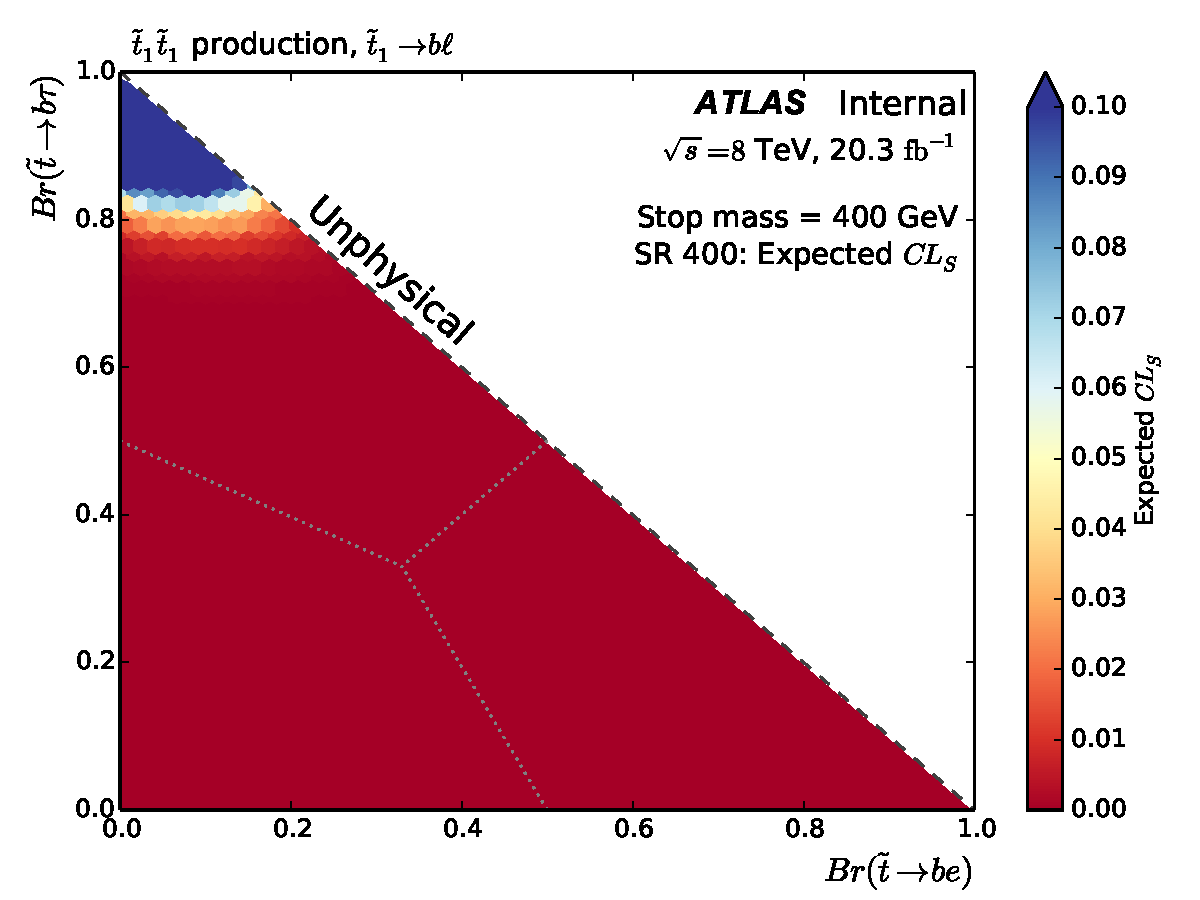
\includegraphics[width=0.65\textwidth]
      {figs/blstop/cls_plots/cls_vs_br_m_400_sr_400_exp.pdf}
  }
  \subbottom[Expected $CL_S$ for SR~600]{
    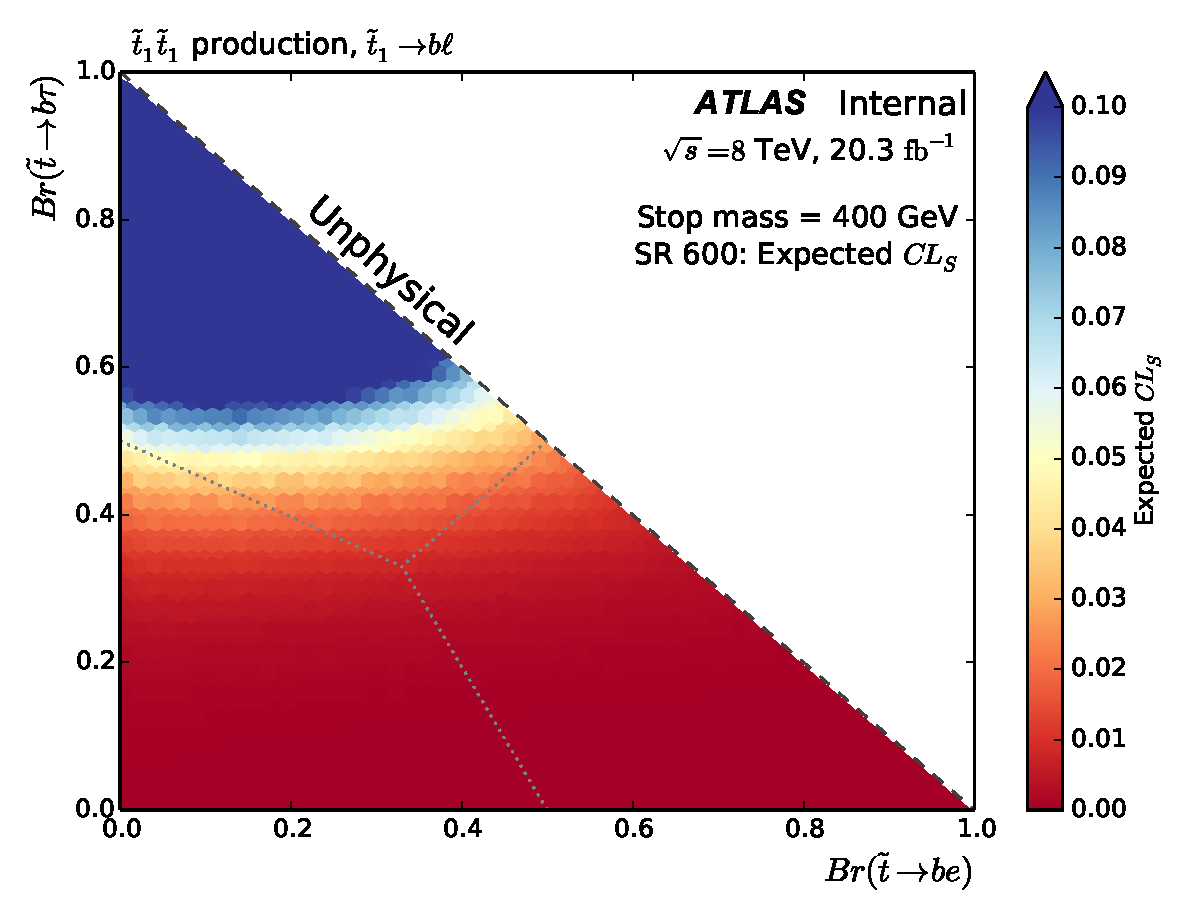
\includegraphics[width=0.65\textwidth]
      {figs/blstop/cls_plots/cls_vs_br_m_400_sr_600_exp.pdf}
  }
  \caption{
    Expected
    $CL_S$ values for SR~400 (top) and SR~600 (bottom) for a stop mass of
    400~\GeV,
    shown across the plane of physical stop branching ratios.
  }
\end{figure}

\begin{figure}[ht]
  \centering
  \subbottom[Observed $CL_S$ for SR~400]{
    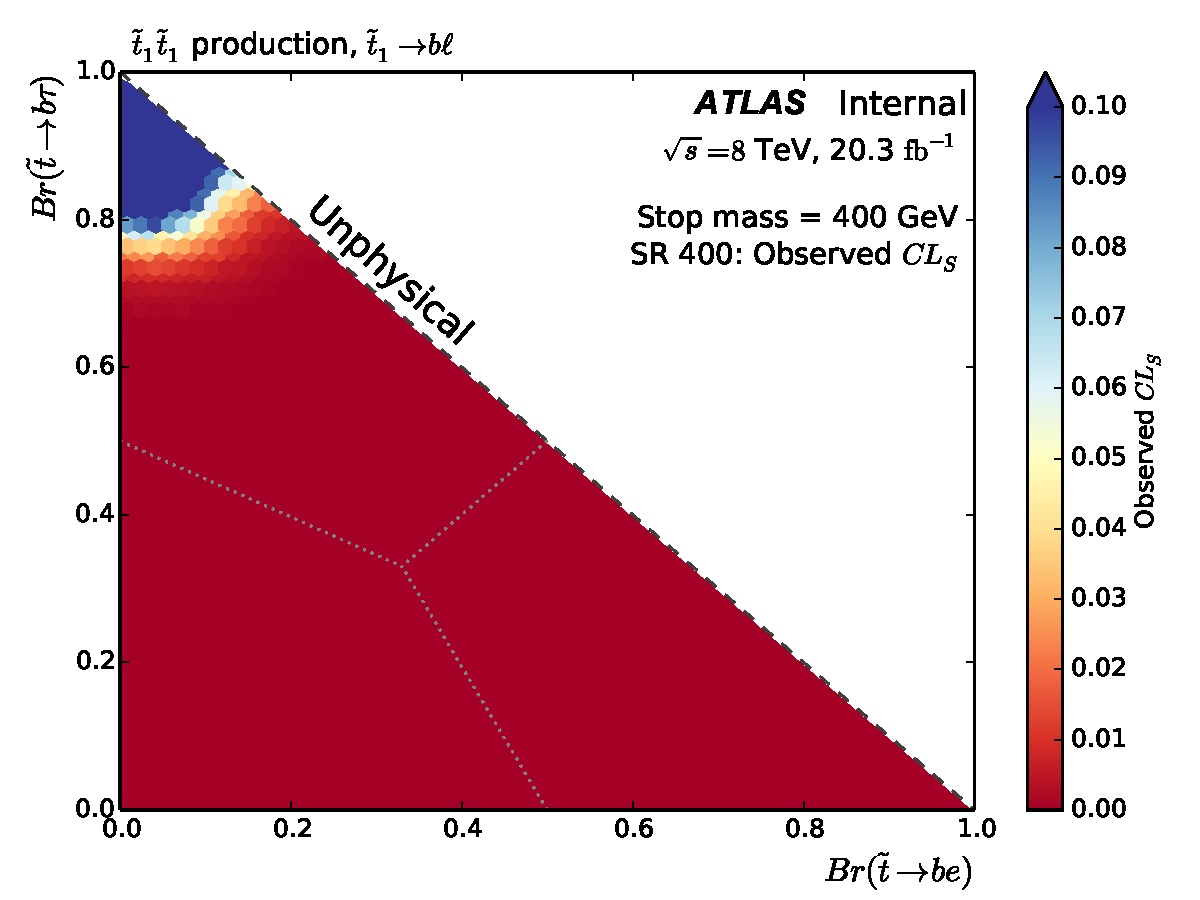
\includegraphics[width=0.65\textwidth]
      {figs/blstop/cls_plots/cls_vs_br_m_400_sr_400_obs.pdf}
  }
  \subbottom[Observed $CL_S$ for SR~600]{
    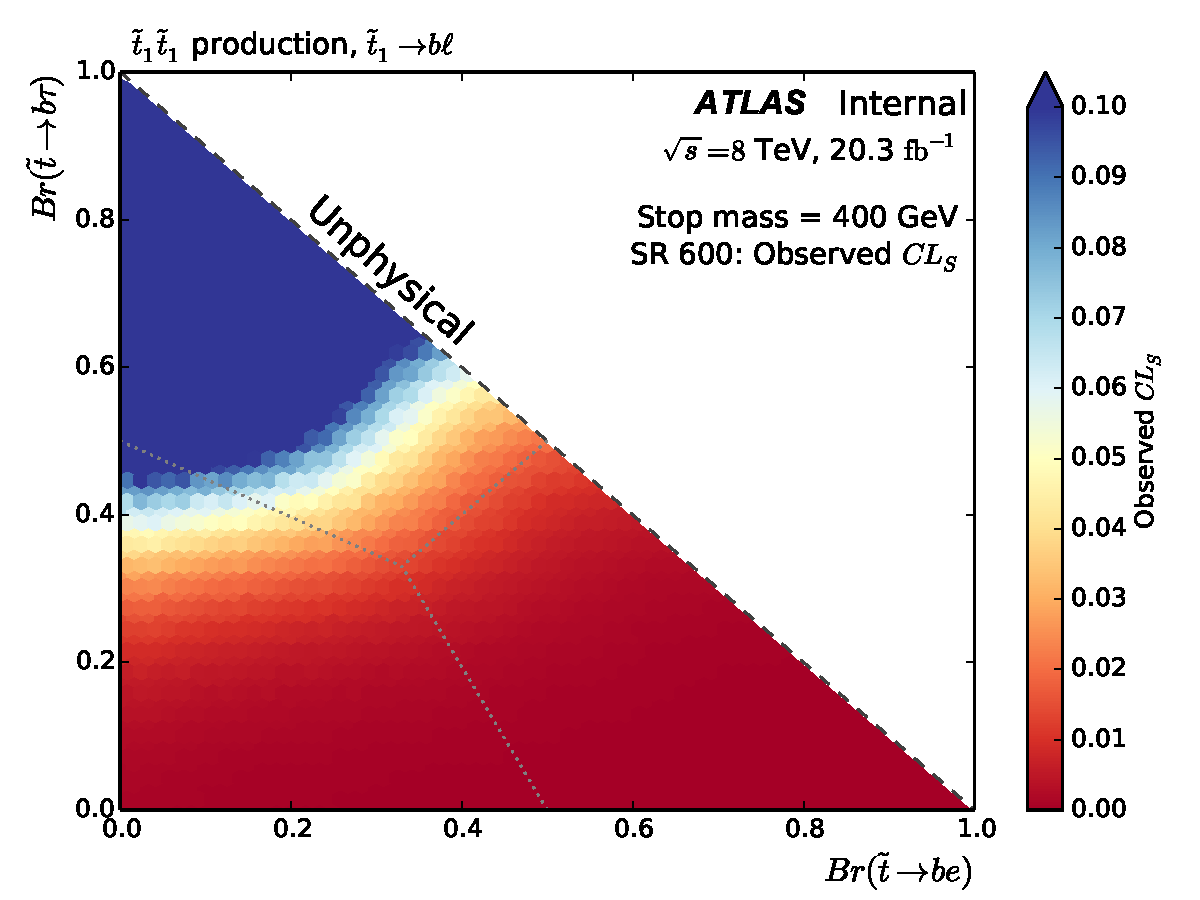
\includegraphics[width=0.65\textwidth]
      {figs/blstop/cls_plots/cls_vs_br_m_400_sr_600_obs.pdf}
  }
  \caption{
    Observed
    $CL_S$ values for SR~400 (top) and SR~600 (bottom) for a stop mass of
    400~\GeV,
    shown across the plane of physical stop branching ratios.
  }
\end{figure}

\begin{figure}[ht]
  \centering
  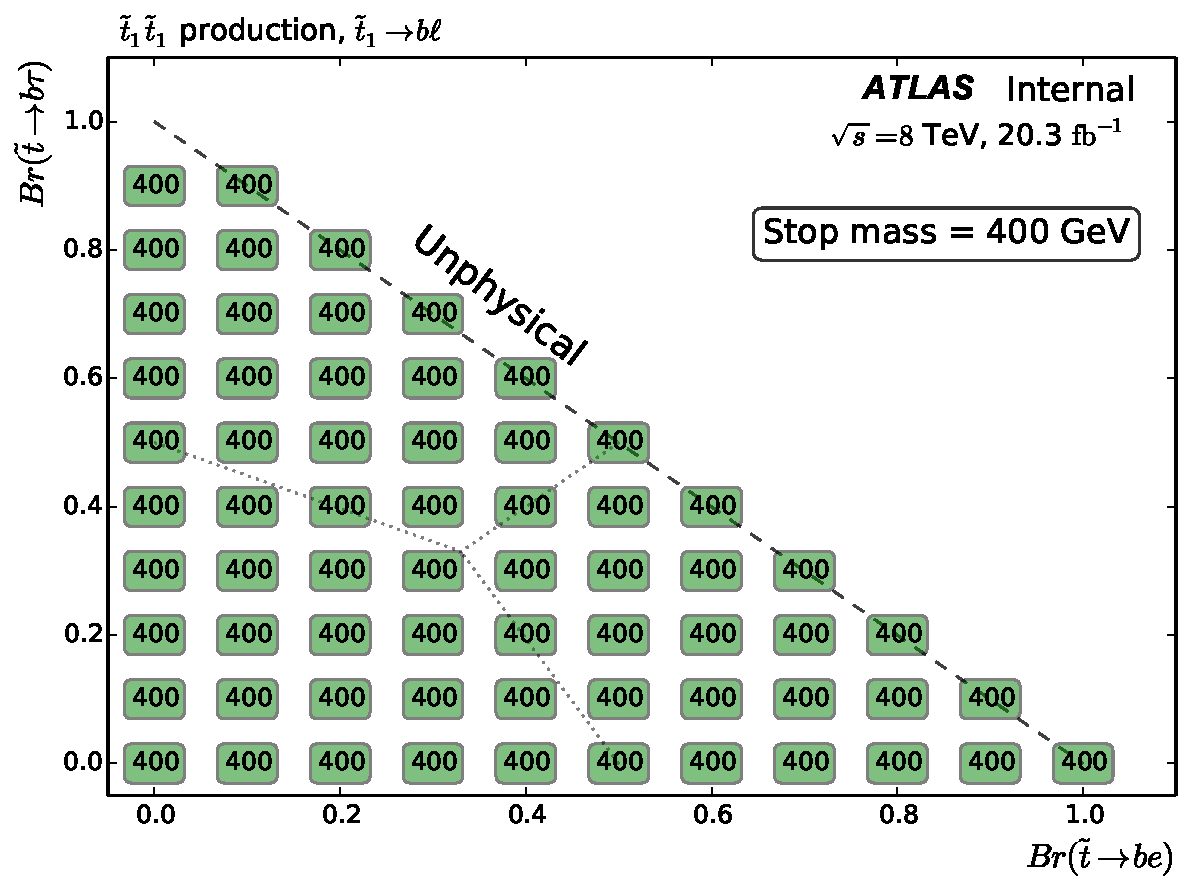
\includegraphics[width=0.85\textwidth]
    {figs/blstop/region_selection/region_choice_vs_br_m_400.pdf}
  \caption{
    SR selection for a stop mass of 400~\GeV.
  }
\end{figure}

\FloatBarrier

%% -----------------------------------------------------------------------------
\newpage
\section{500 GeV stop mass}

\begin{figure}[ht]
  \centering
  \subbottom[Expected $CL_S$ for SR~400]{
    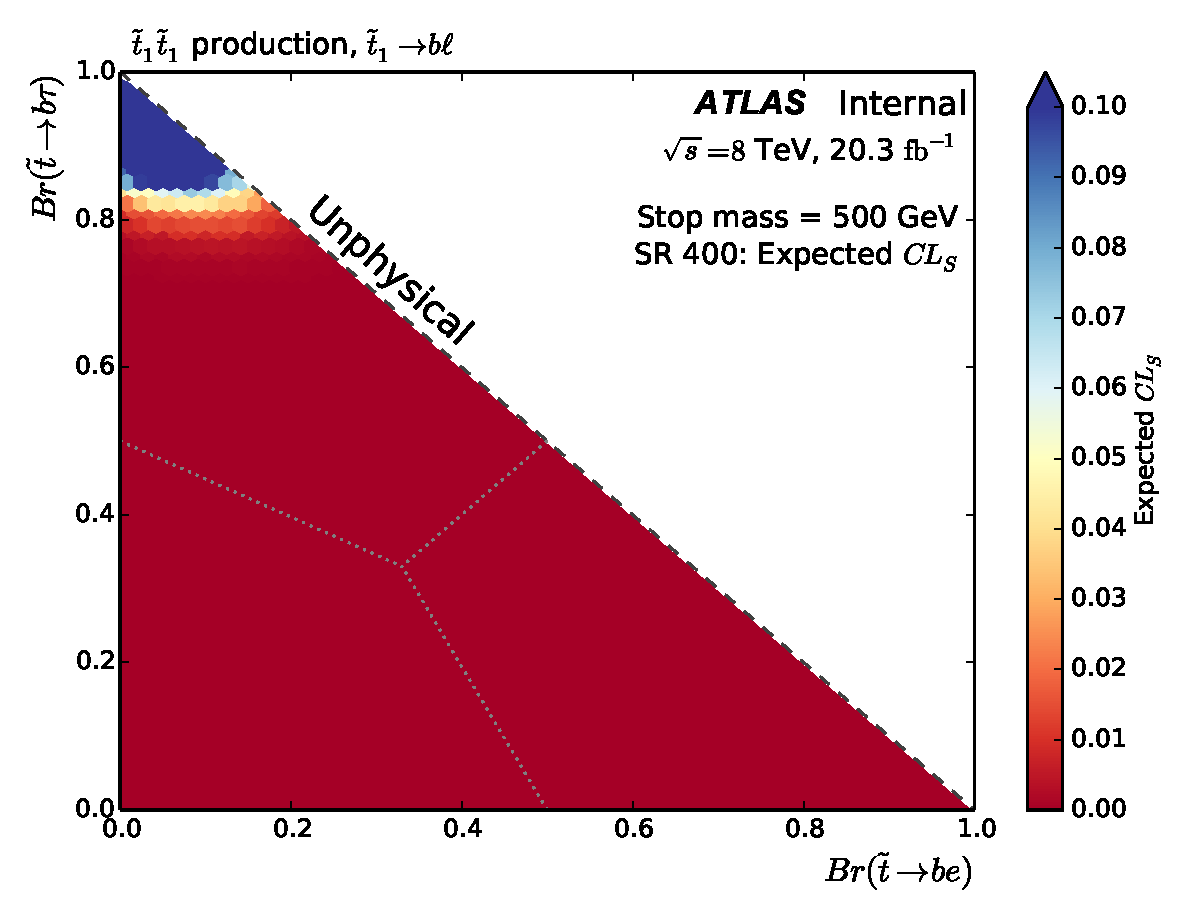
\includegraphics[width=0.65\textwidth]
      {figs/blstop/cls_plots/cls_vs_br_m_500_sr_400_exp.pdf}
  }
  \subbottom[Expected $CL_S$ for SR~600]{
    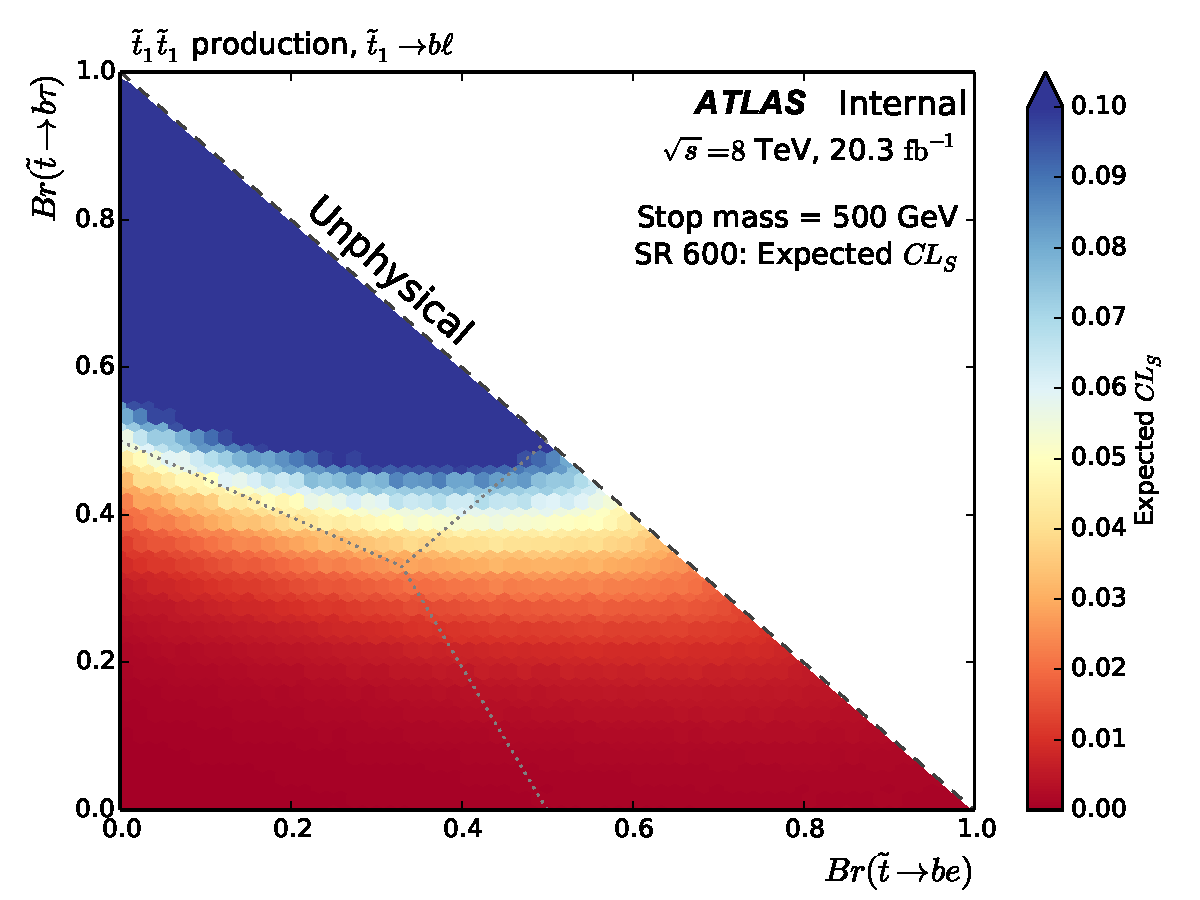
\includegraphics[width=0.65\textwidth]
      {figs/blstop/cls_plots/cls_vs_br_m_500_sr_600_exp.pdf}
  }
  \caption{
    Expected
    $CL_S$ values for SR~400 (top) and SR~600 (bottom) for a stop mass of
    500~\GeV,
    shown across the plane of physical stop branching ratios.
  }
\end{figure}

\begin{figure}[ht]
  \centering
  \subbottom[Observed $CL_S$ for SR~400]{
    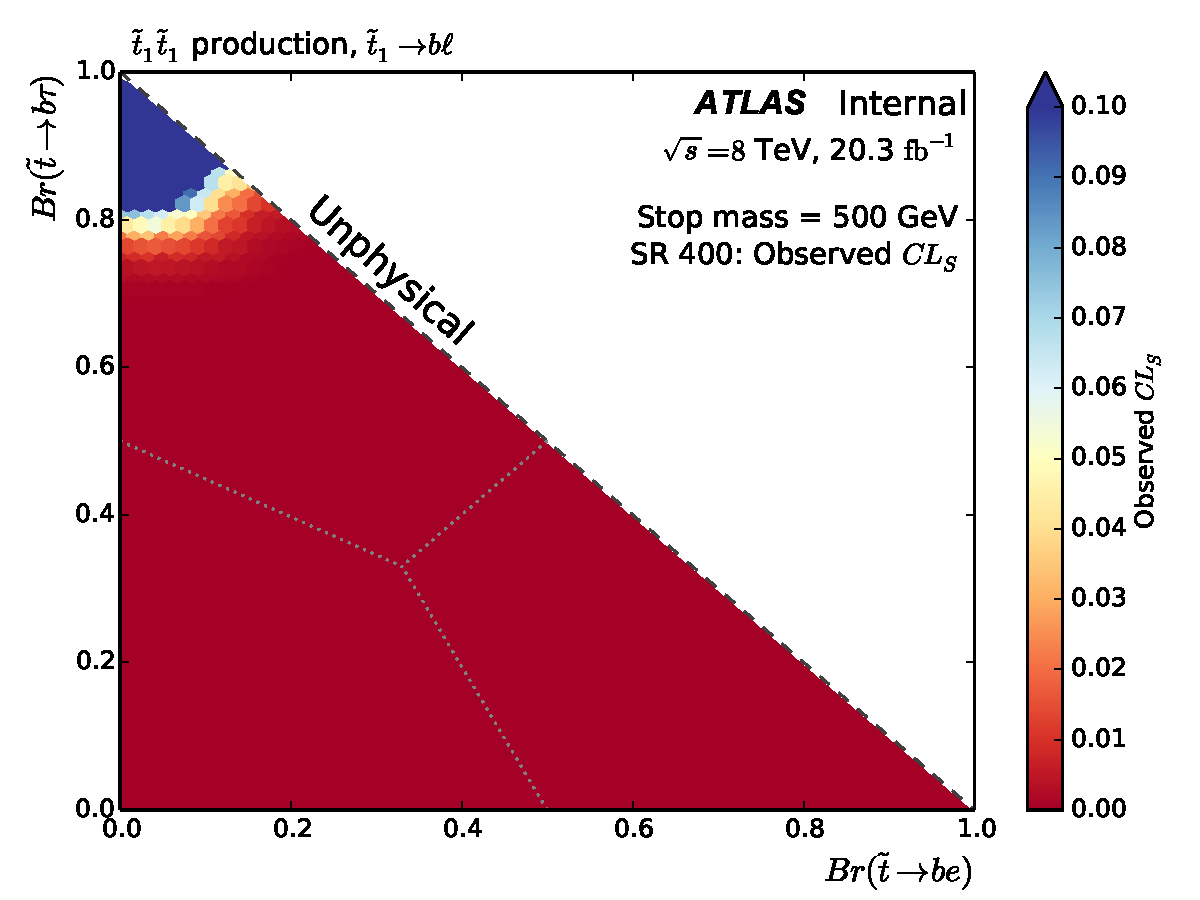
\includegraphics[width=0.65\textwidth]
      {figs/blstop/cls_plots/cls_vs_br_m_500_sr_400_obs.pdf}
  }
  \subbottom[Observed $CL_S$ for SR~600]{
    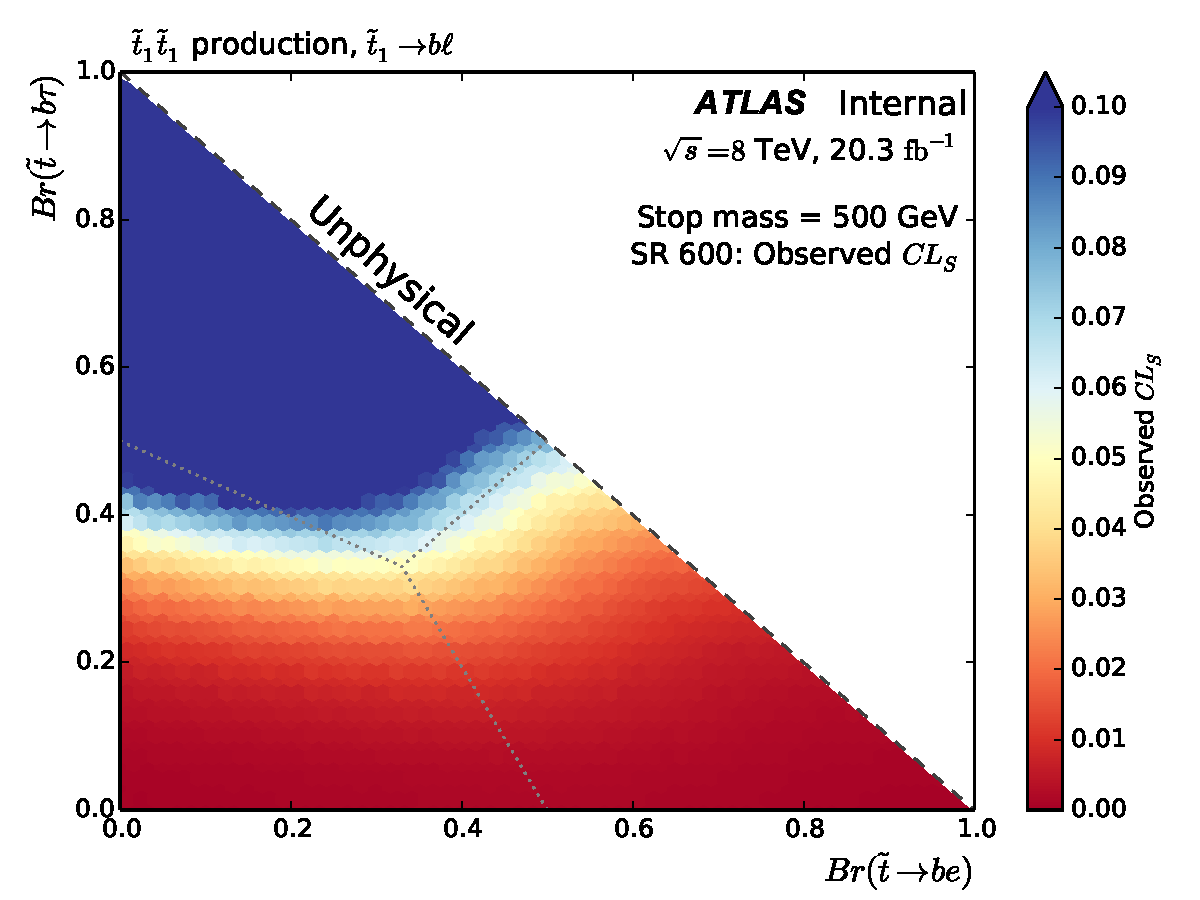
\includegraphics[width=0.65\textwidth]
      {figs/blstop/cls_plots/cls_vs_br_m_500_sr_600_obs.pdf}
  }
  \caption{
    Observed
    $CL_S$ values for SR~400 (top) and SR~600 (bottom) for a stop mass of
    500~\GeV,
    shown across the plane of physical stop branching ratios.
  }
\end{figure}

\begin{figure}[ht]
  \centering
  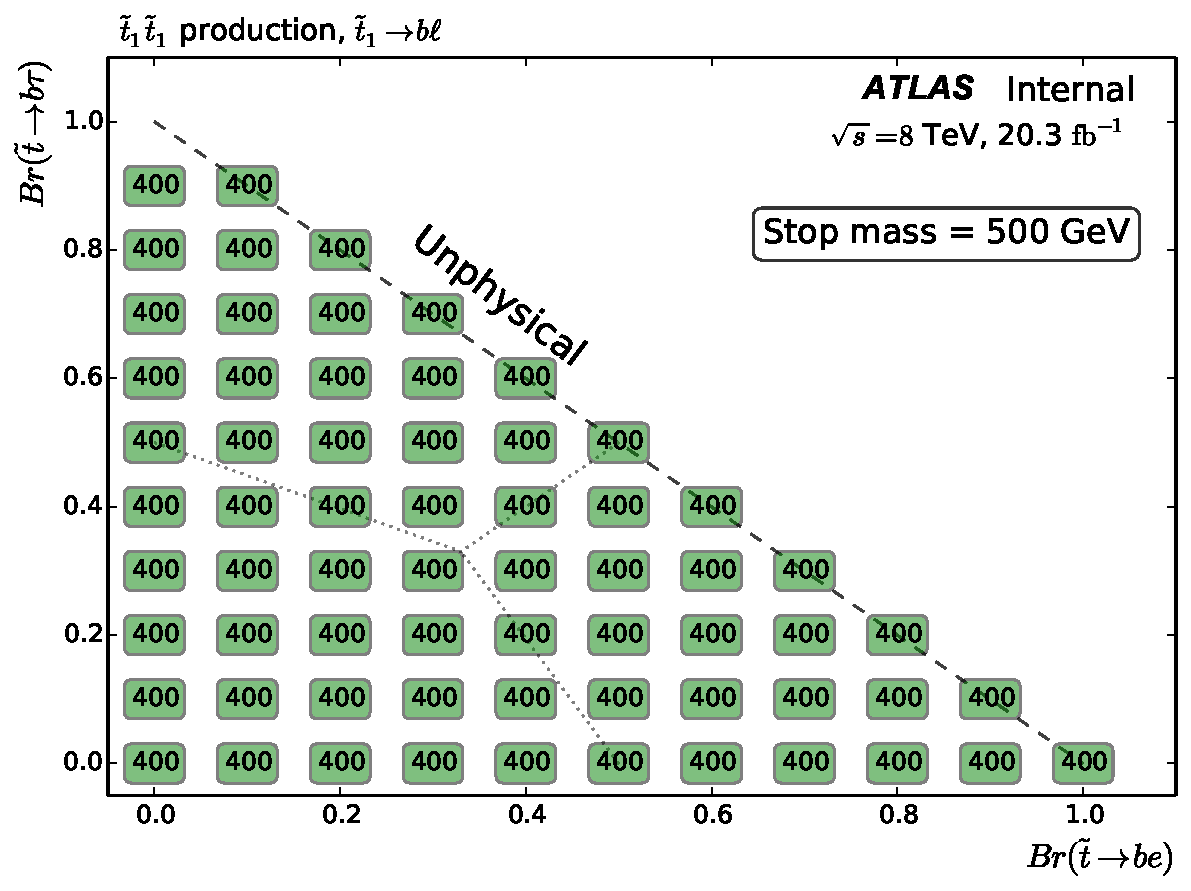
\includegraphics[width=0.85\textwidth]
    {figs/blstop/region_selection/region_choice_vs_br_m_500.pdf}
  \caption{
    SR selection for a stop mass of 500~\GeV.
  }
\end{figure}

\FloatBarrier

%% -----------------------------------------------------------------------------
\newpage
\section{600 GeV stop mass}

\begin{figure}[ht]
  \centering
  \subbottom[Expected $CL_S$ for SR~400]{
    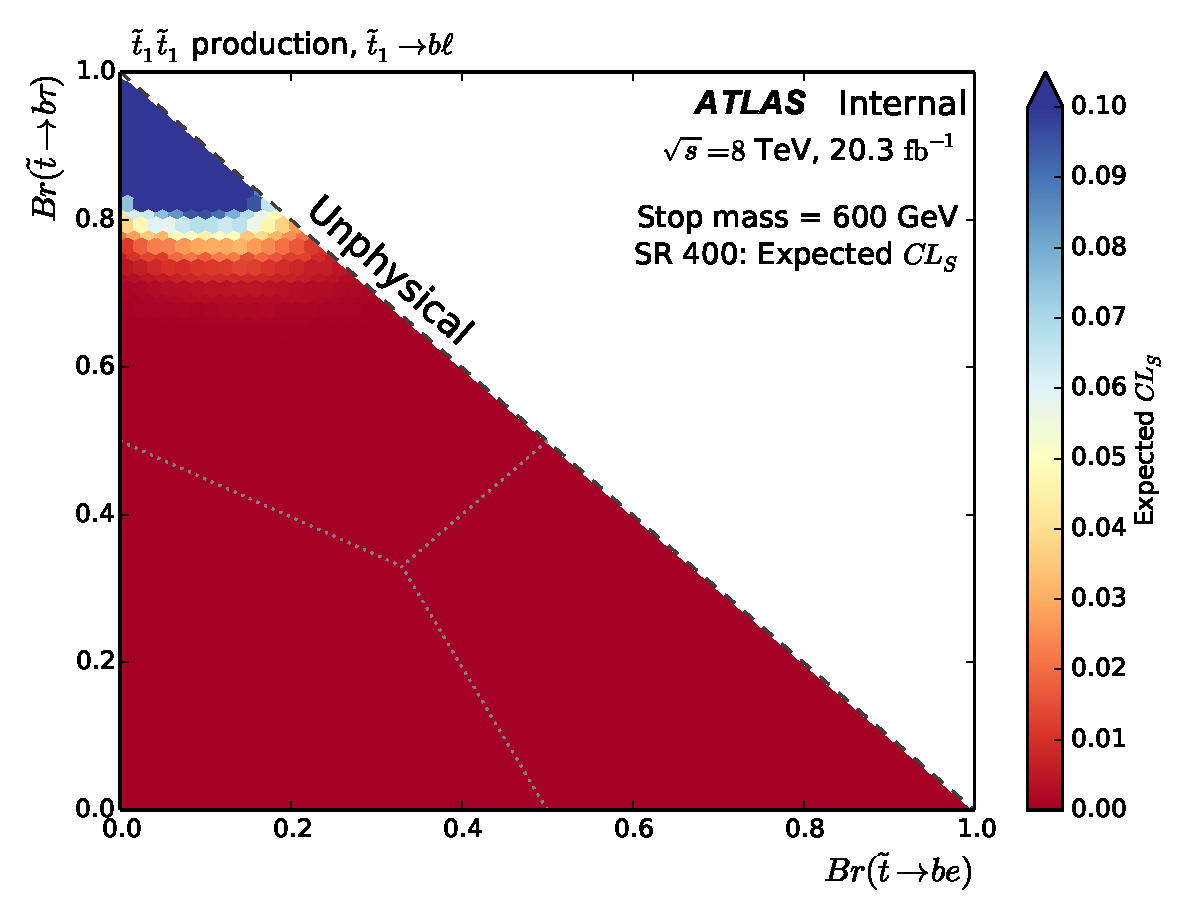
\includegraphics[width=0.65\textwidth]
      {figs/blstop/cls_plots/cls_vs_br_m_600_sr_400_exp.pdf}
  }
  \subbottom[Expected $CL_S$ for SR~600]{
    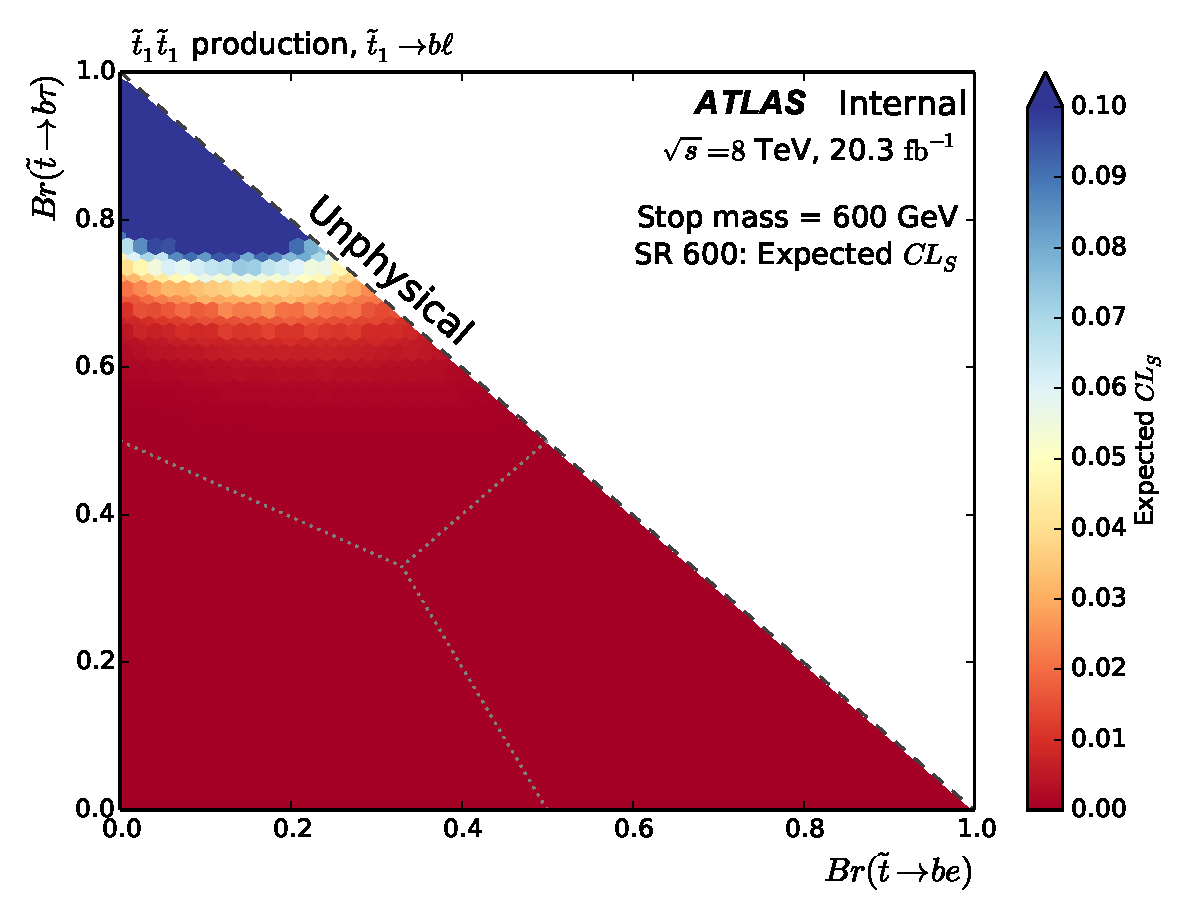
\includegraphics[width=0.65\textwidth]
      {figs/blstop/cls_plots/cls_vs_br_m_600_sr_600_exp.pdf}
  }
  \caption{
    Expected
    $CL_S$ values for SR~400 (top) and SR~600 (bottom) for a stop mass of
    600~\GeV,
    shown across the plane of physical stop branching ratios.
  }
\end{figure}

\begin{figure}[ht]
  \centering
  \subbottom[Observed $CL_S$ for SR~400]{
    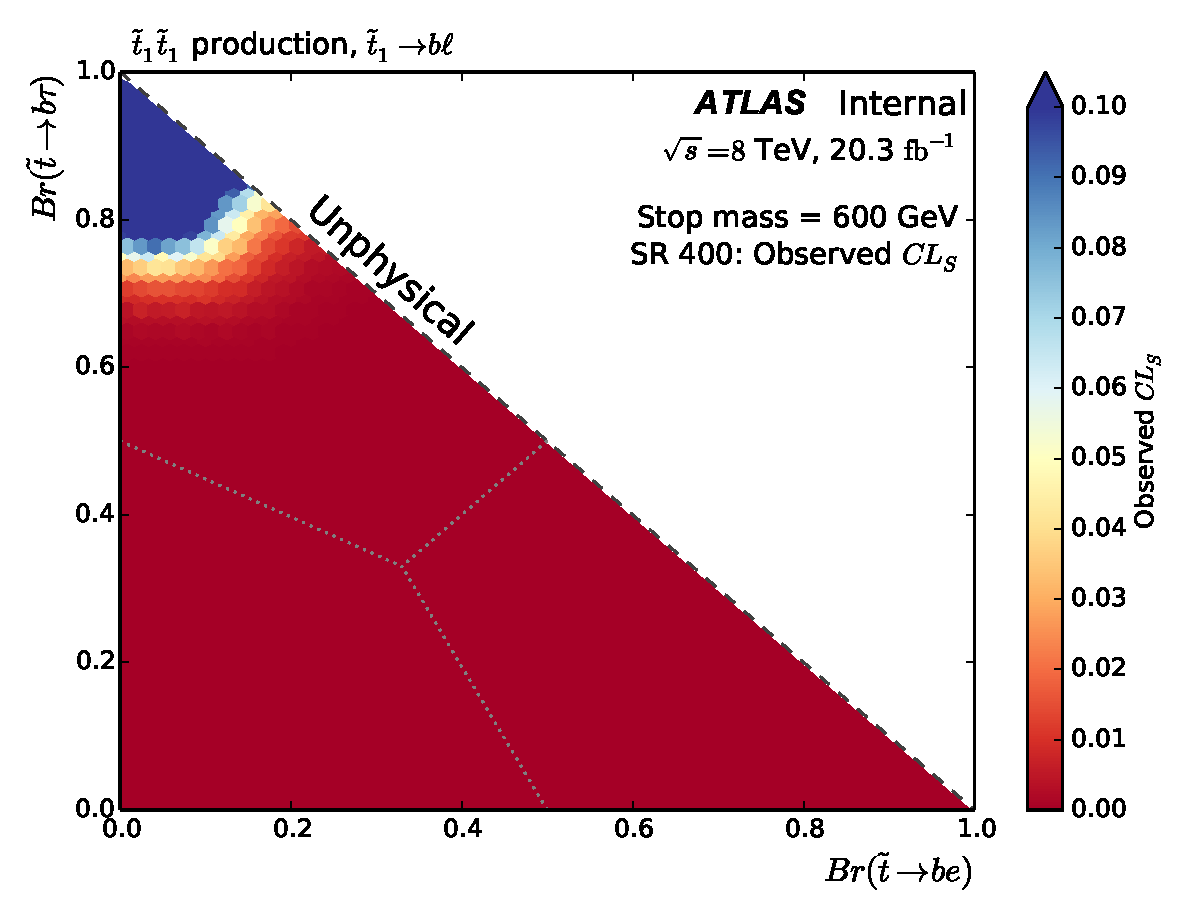
\includegraphics[width=0.65\textwidth]
      {figs/blstop/cls_plots/cls_vs_br_m_600_sr_400_obs.pdf}
  }
  \subbottom[Observed $CL_S$ for SR~600]{
    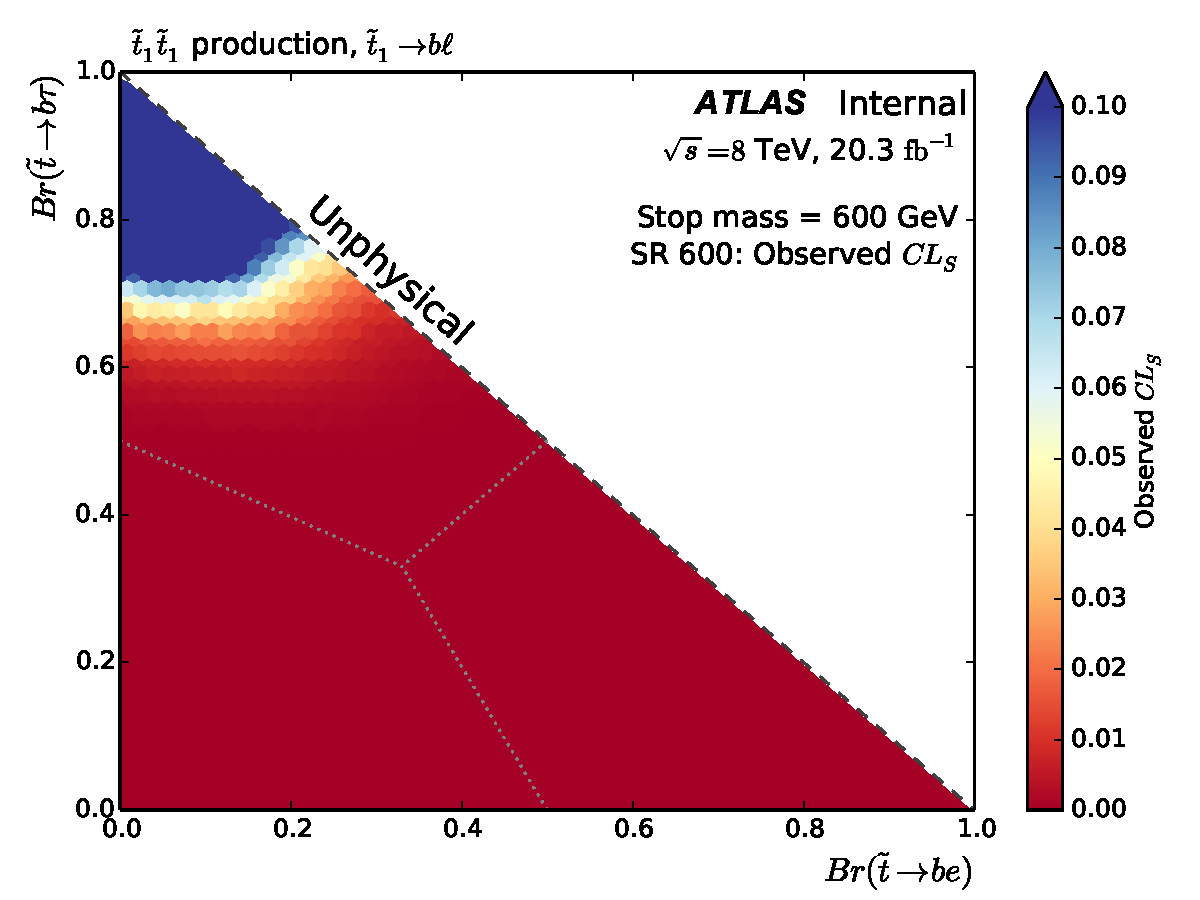
\includegraphics[width=0.65\textwidth]
      {figs/blstop/cls_plots/cls_vs_br_m_600_sr_600_obs.pdf}
  }
  \caption{
    Observed
    $CL_S$ values for SR~400 (top) and SR~600 (bottom) for a stop mass of
    600~\GeV,
    shown across the plane of physical stop branching ratios.
  }
\end{figure}

\begin{figure}[ht]
  \centering
  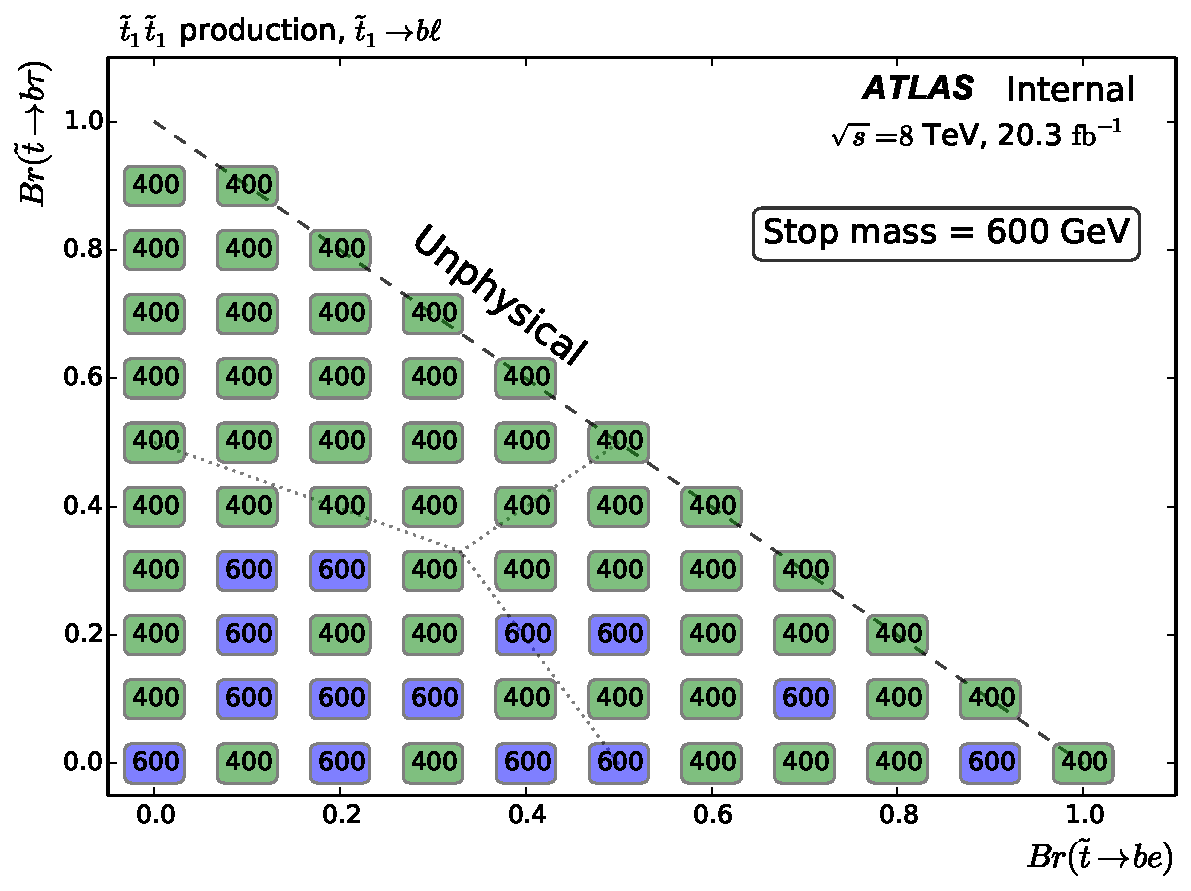
\includegraphics[width=0.85\textwidth]
    {figs/blstop/region_selection/region_choice_vs_br_m_600.pdf}
  \caption{
    SR selection for a stop mass of 600~\GeV.
  }
\end{figure}

\FloatBarrier

%% -----------------------------------------------------------------------------
\newpage
\section{700 GeV stop mass}

\begin{figure}[ht]
  \centering
  \subbottom[Expected $CL_S$ for SR~400]{
    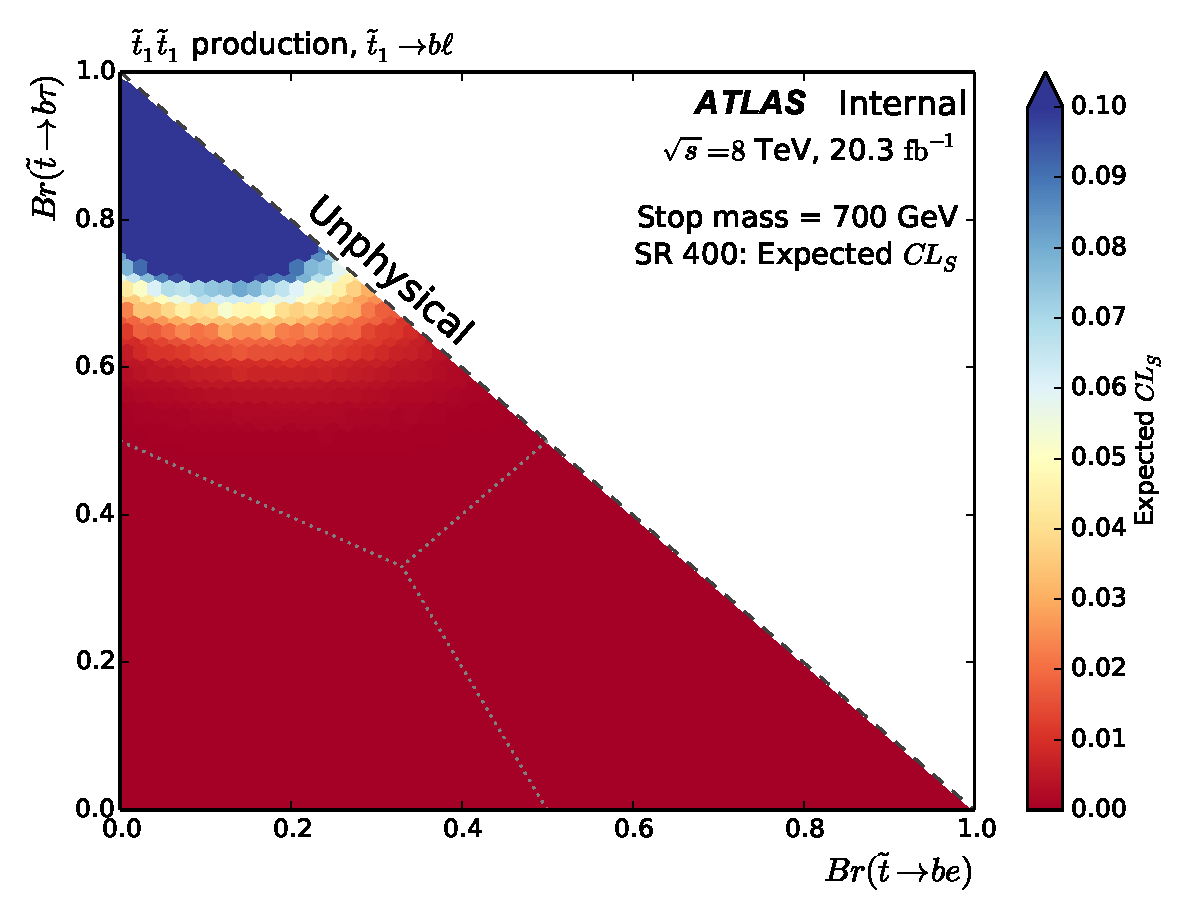
\includegraphics[width=0.65\textwidth]
      {figs/blstop/cls_plots/cls_vs_br_m_700_sr_400_exp.pdf}
  }
  \subbottom[Expected $CL_S$ for SR~600]{
    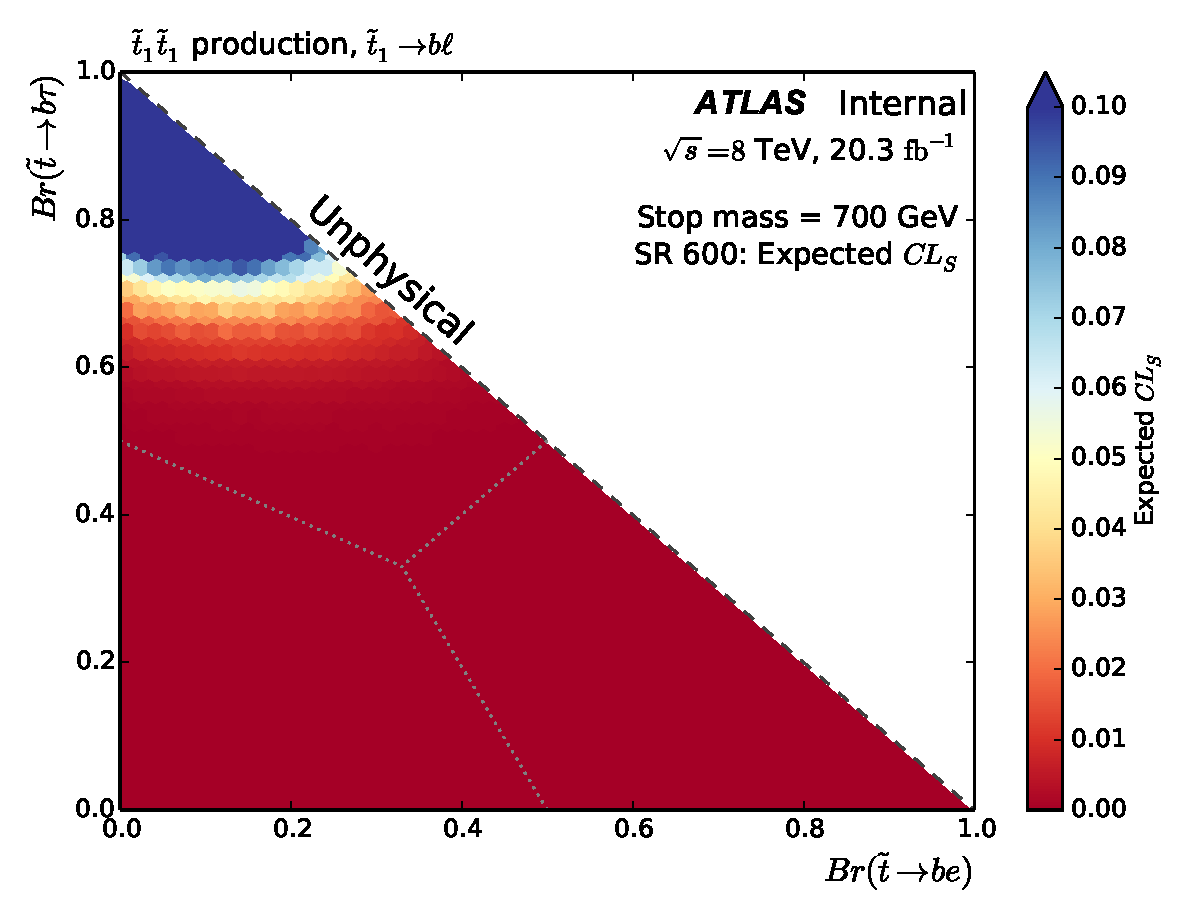
\includegraphics[width=0.65\textwidth]
      {figs/blstop/cls_plots/cls_vs_br_m_700_sr_600_exp.pdf}
  }
  \caption{
    Expected
    $CL_S$ values for SR~400 (top) and SR~600 (bottom) for a stop mass of
    700~\GeV,
    shown across the plane of physical stop branching ratios.
  }
\end{figure}

\begin{figure}[ht]
  \centering
  \subbottom[Observed $CL_S$ for SR~400]{
    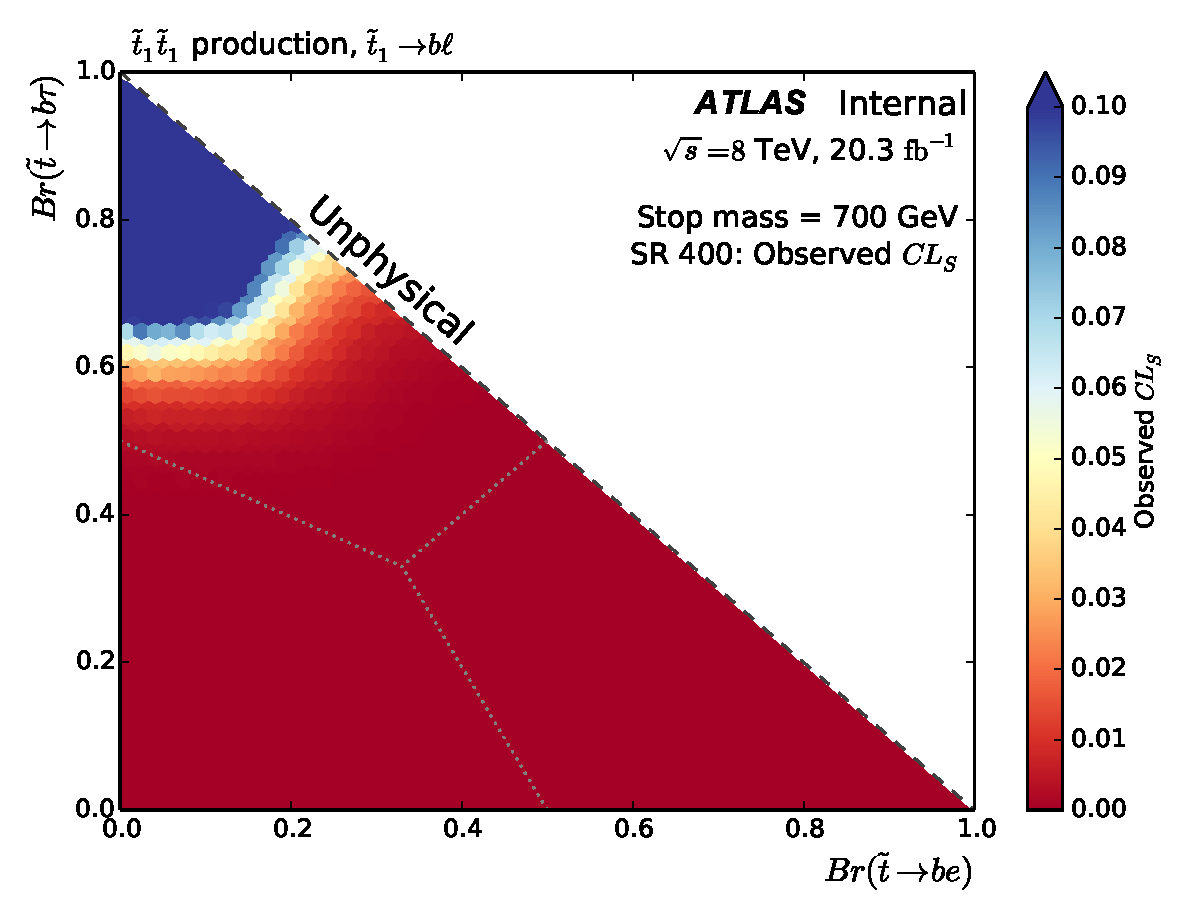
\includegraphics[width=0.65\textwidth]
      {figs/blstop/cls_plots/cls_vs_br_m_700_sr_400_obs.pdf}
  }
  \subbottom[Observed $CL_S$ for SR~600]{
    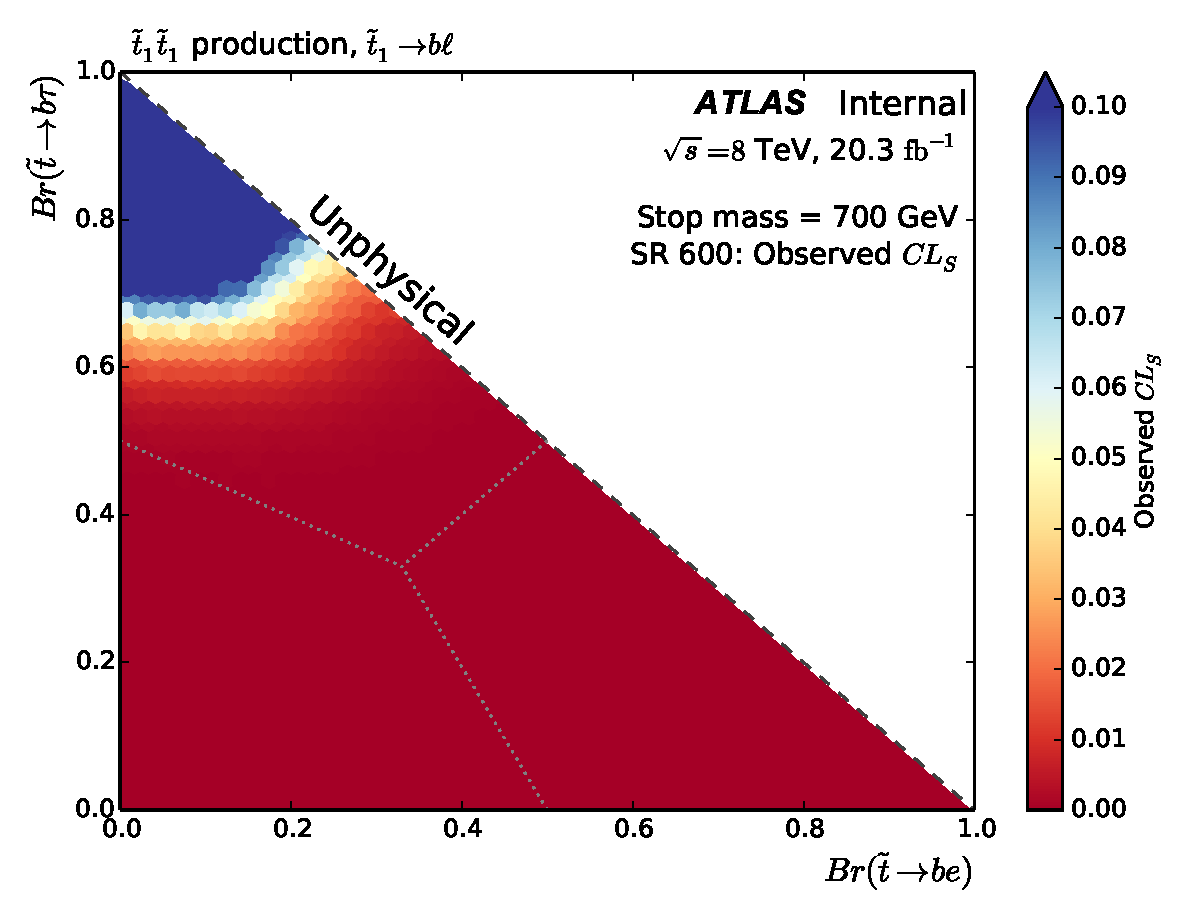
\includegraphics[width=0.65\textwidth]
      {figs/blstop/cls_plots/cls_vs_br_m_700_sr_600_obs.pdf}
  }
  \caption{
    Observed
    $CL_S$ values for SR~400 (top) and SR~600 (bottom) for a stop mass of
    700~\GeV,
    shown across the plane of physical stop branching ratios.
  }
\end{figure}

\begin{figure}[ht]
  \centering
  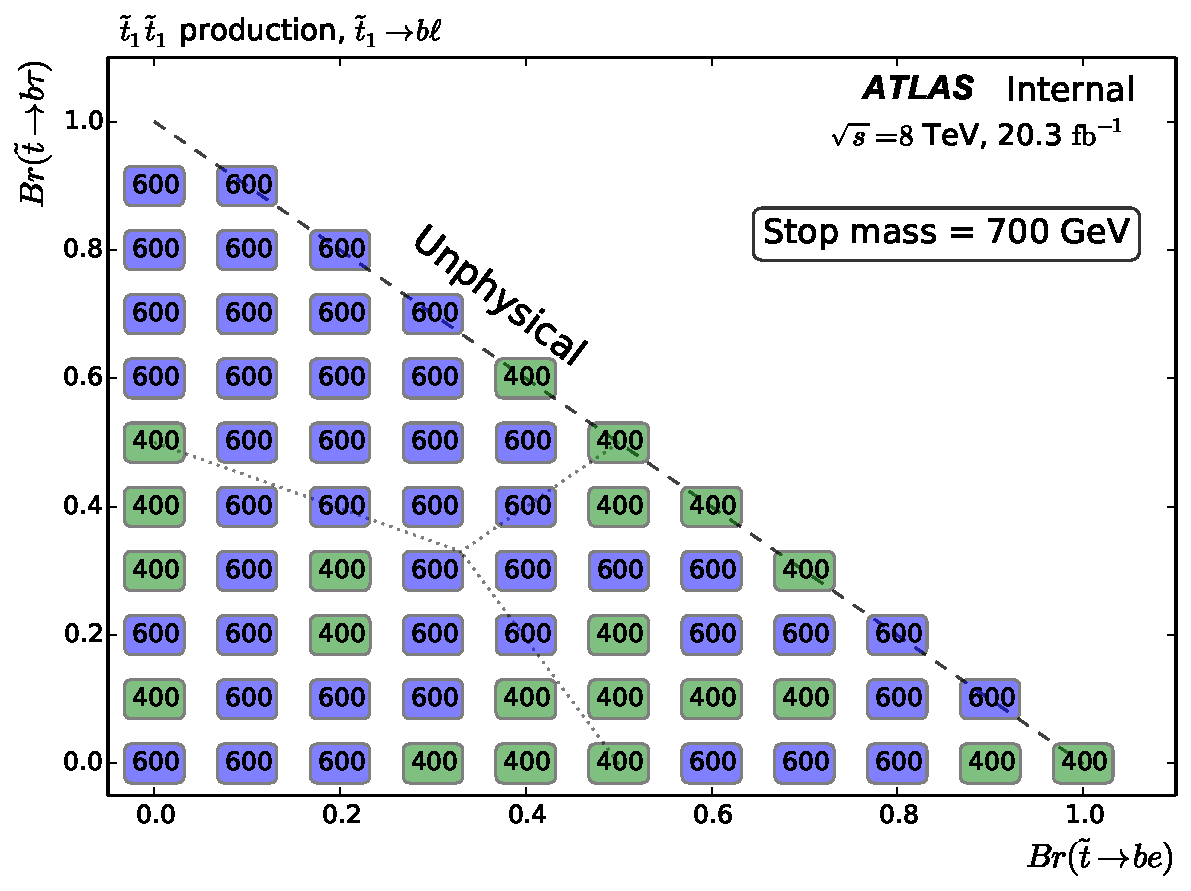
\includegraphics[width=0.85\textwidth]
    {figs/blstop/region_selection/region_choice_vs_br_m_700.pdf}
  \caption{
    SR selection for a stop mass of 700~\GeV.
  }
\end{figure}

\FloatBarrier

%% -----------------------------------------------------------------------------
\newpage
\section{800 GeV stop mass}

\begin{figure}[ht]
  \centering
  \subbottom[Expected $CL_S$ for SR~400]{
    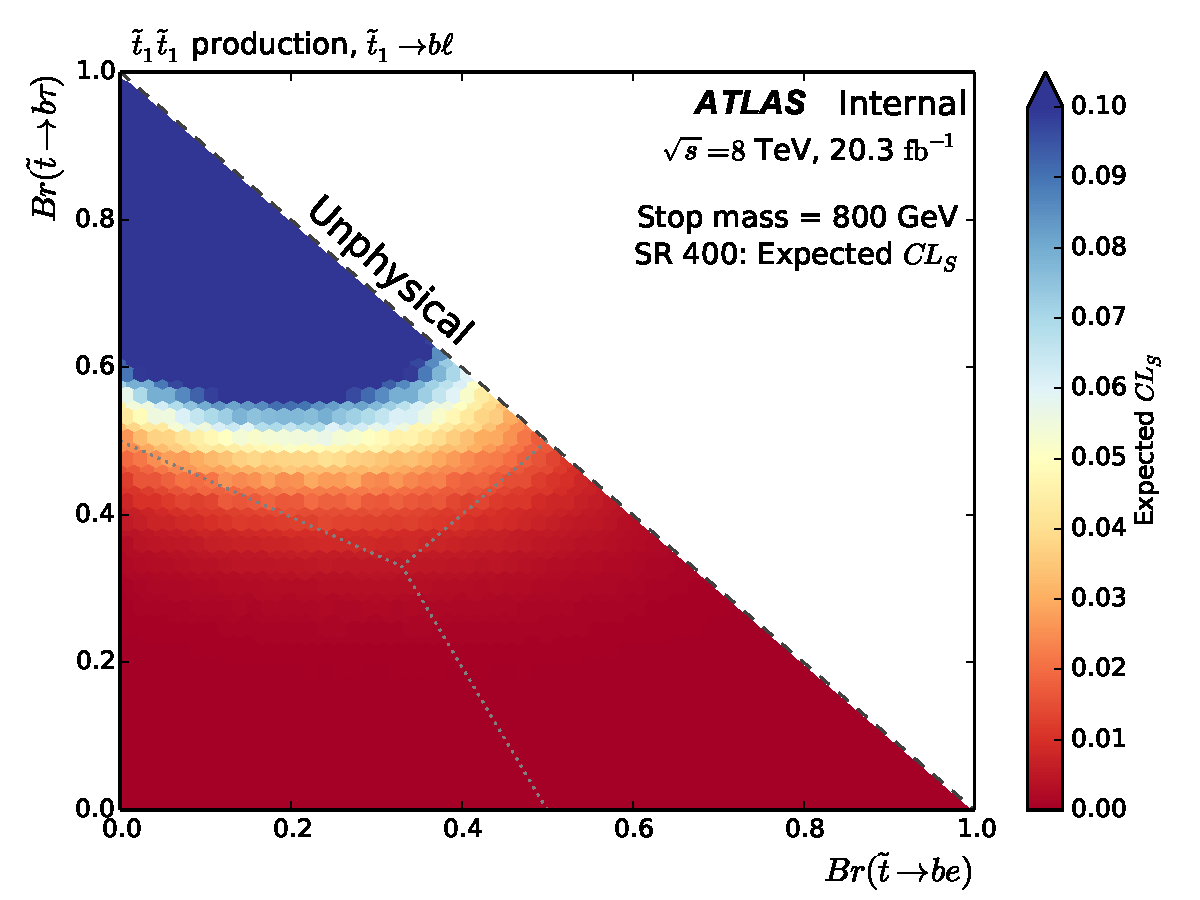
\includegraphics[width=0.65\textwidth]
      {figs/blstop/cls_plots/cls_vs_br_m_800_sr_400_exp.pdf}
  }
  \subbottom[Expected $CL_S$ for SR~600]{
    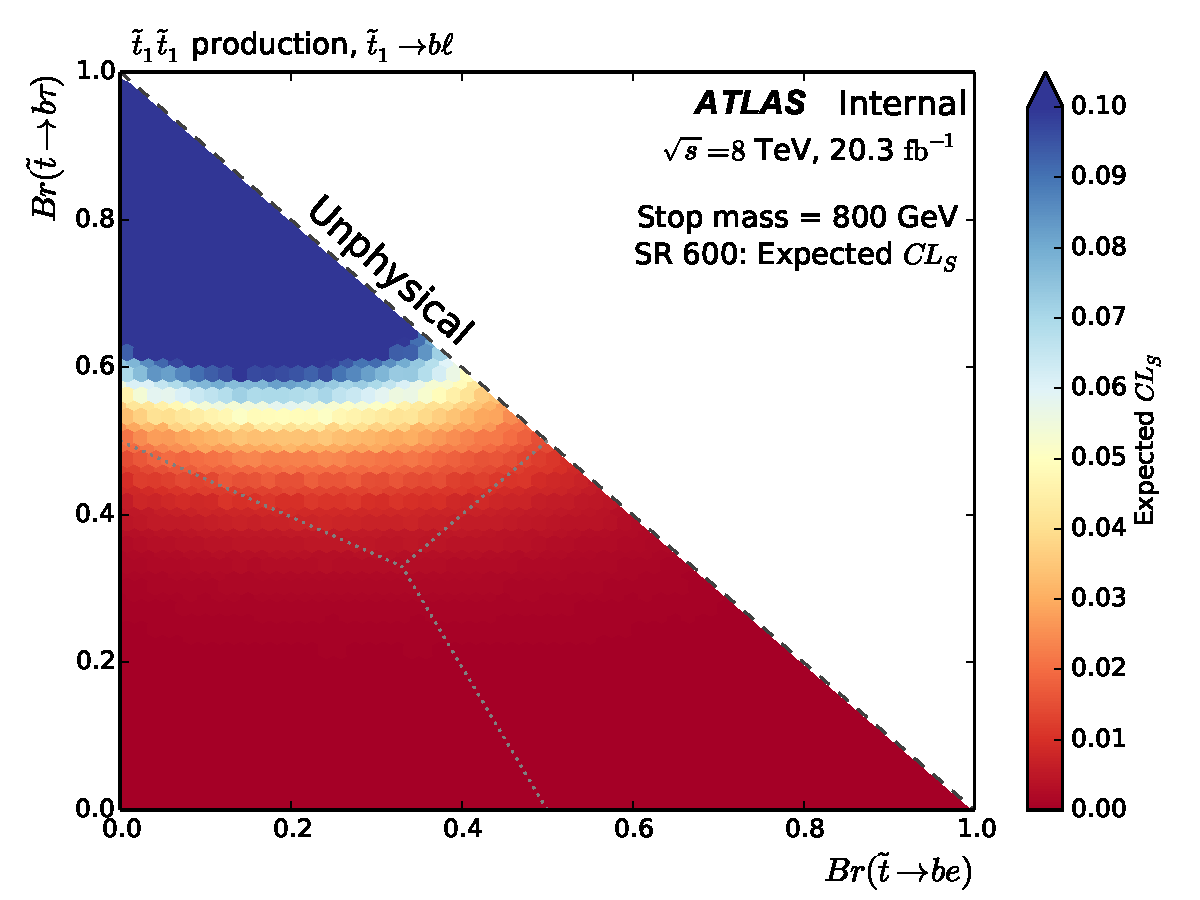
\includegraphics[width=0.65\textwidth]
      {figs/blstop/cls_plots/cls_vs_br_m_800_sr_600_exp.pdf}
  }
  \caption{
    Expected
    $CL_S$ values for SR~400 (top) and SR~600 (bottom) for a stop mass of
    800~\GeV,
    shown across the plane of physical stop branching ratios.
  }
\end{figure}

\begin{figure}[ht]
  \centering
  \subbottom[Observed $CL_S$ for SR~400]{
    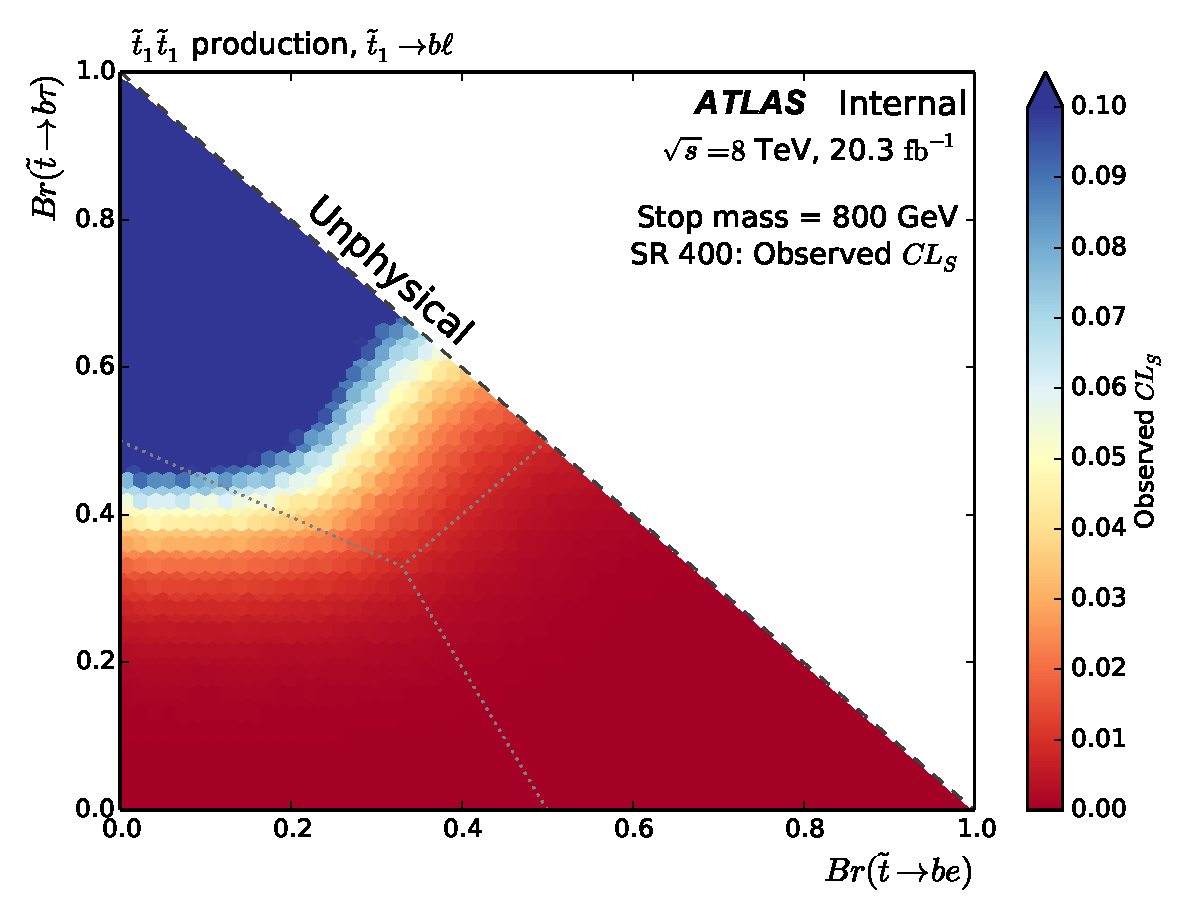
\includegraphics[width=0.65\textwidth]
      {figs/blstop/cls_plots/cls_vs_br_m_800_sr_400_obs.pdf}
  }
  \subbottom[Observed $CL_S$ for SR~600]{
    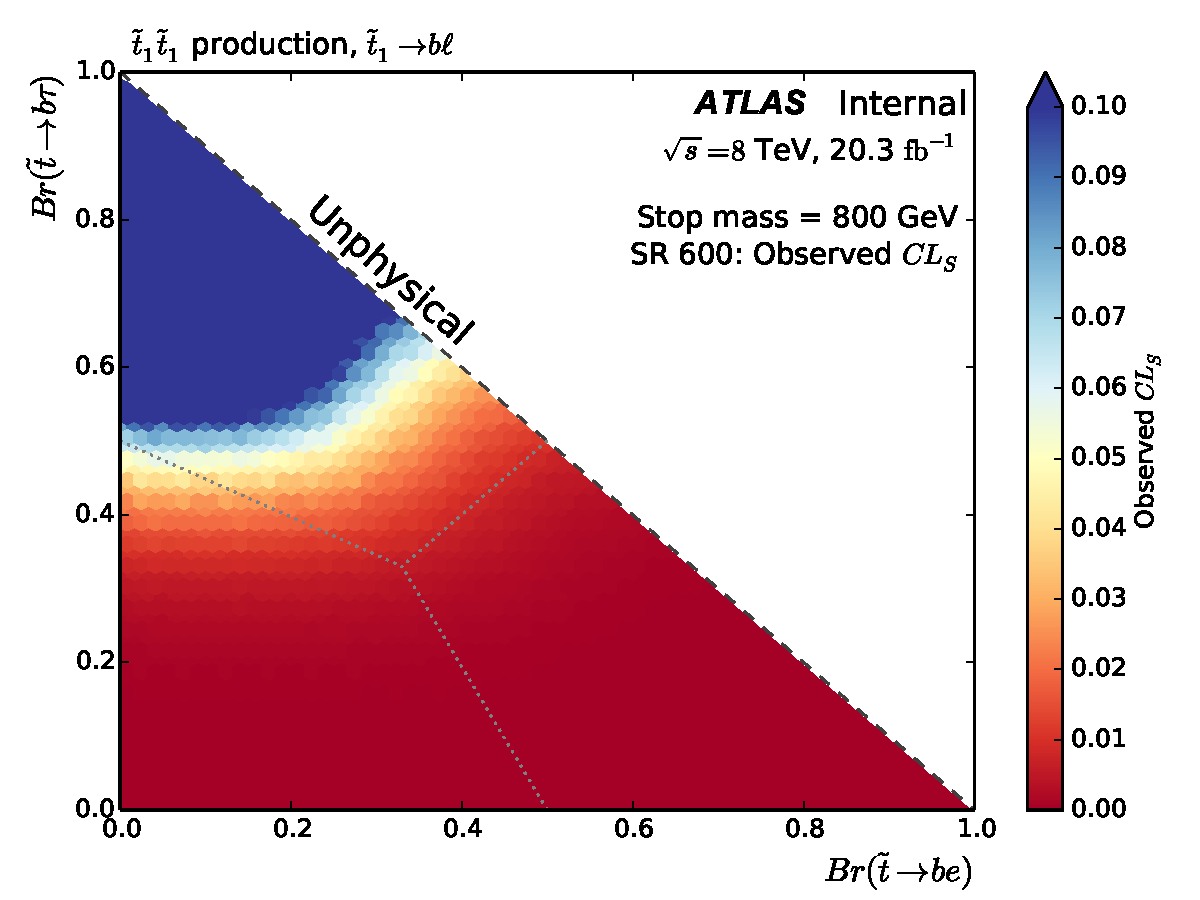
\includegraphics[width=0.65\textwidth]
      {figs/blstop/cls_plots/cls_vs_br_m_800_sr_600_obs.pdf}
  }
  \caption{
    Observed
    $CL_S$ values for SR~400 (top) and SR~600 (bottom) for a stop mass of
    800~\GeV,
    shown across the plane of physical stop branching ratios.
  }
\end{figure}

\begin{figure}[ht]
  \centering
  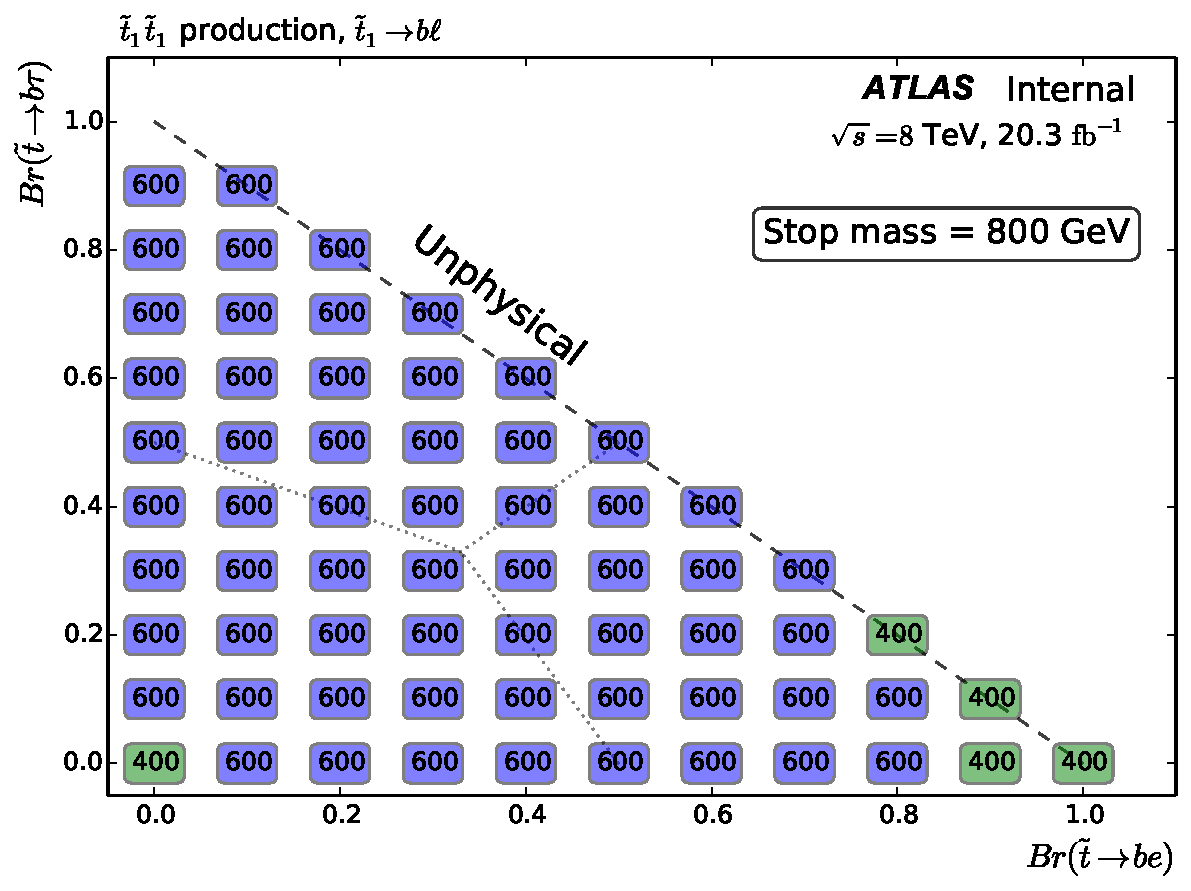
\includegraphics[width=0.85\textwidth]
    {figs/blstop/region_selection/region_choice_vs_br_m_800.pdf}
  \caption{
    SR selection for a stop mass of 800~\GeV.
  }
\end{figure}

\FloatBarrier

%% -----------------------------------------------------------------------------
\newpage
\section{900 GeV stop mass}

\begin{figure}[ht]
  \centering
  \subbottom[Expected $CL_S$ for SR~400]{
    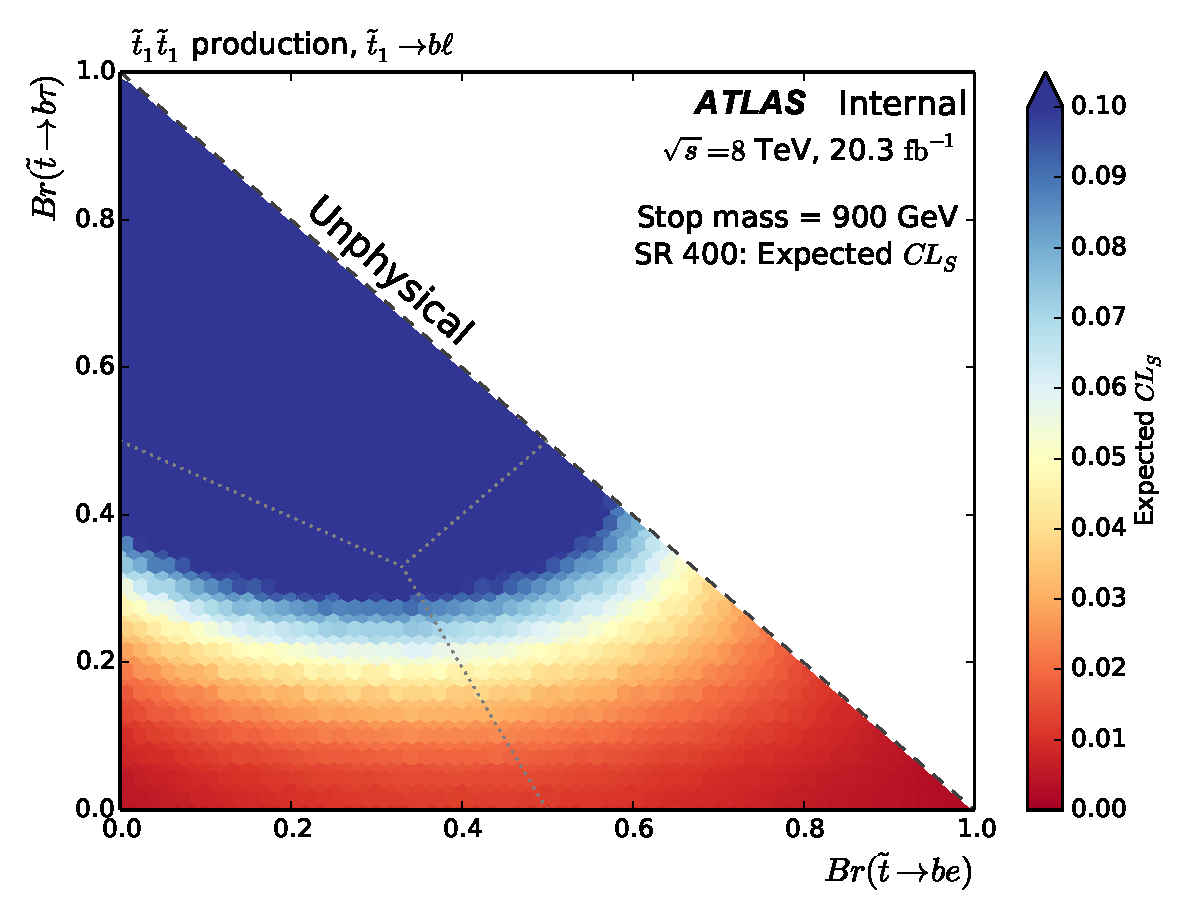
\includegraphics[width=0.65\textwidth]
      {figs/blstop/cls_plots/cls_vs_br_m_900_sr_400_exp.pdf}
  }
  \subbottom[Expected $CL_S$ for SR~600]{
    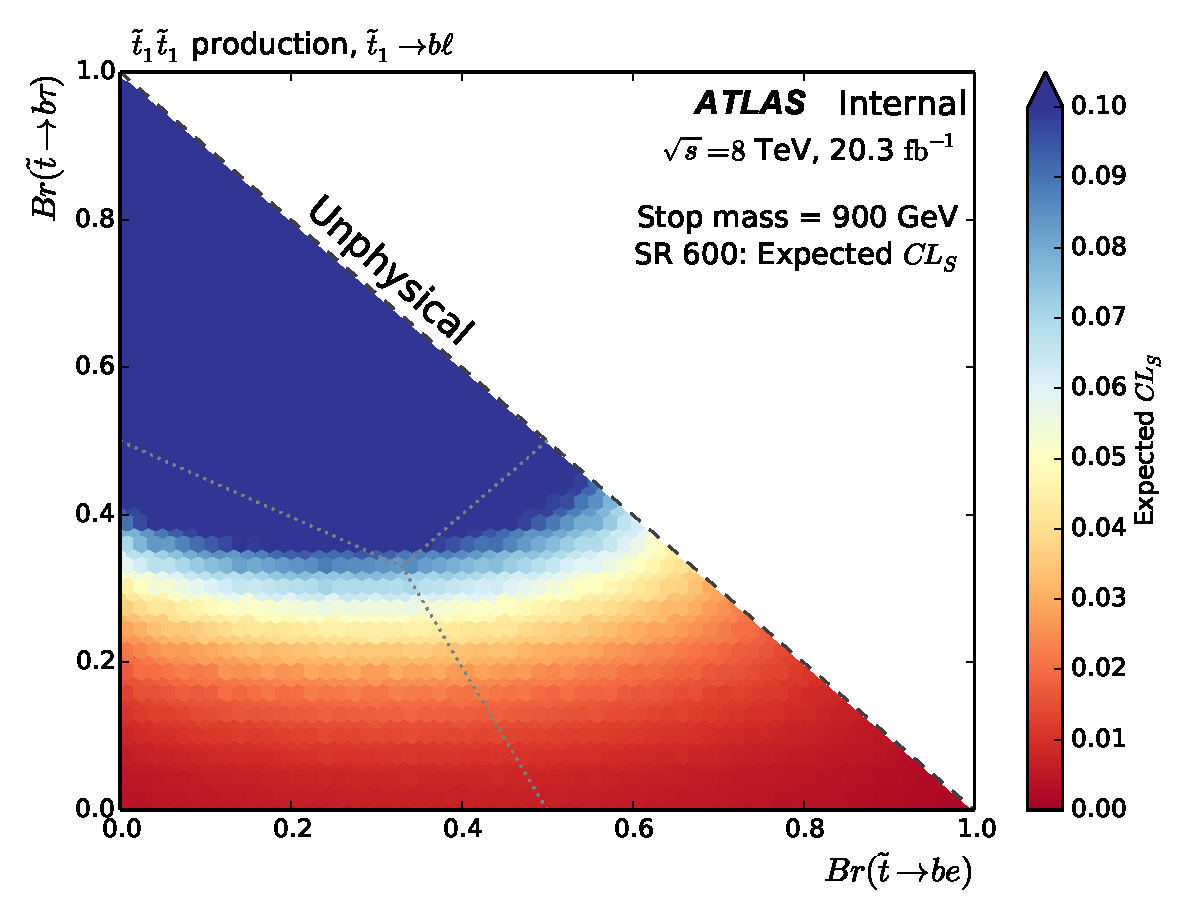
\includegraphics[width=0.65\textwidth]
      {figs/blstop/cls_plots/cls_vs_br_m_900_sr_600_exp.pdf}
  }
  \caption{
    Expected
    $CL_S$ values for SR~400 (top) and SR~600 (bottom) for a stop mass of
    900~\GeV,
    shown across the plane of physical stop branching ratios.
  }
\end{figure}

\begin{figure}[ht]
  \centering
  \subbottom[Observed $CL_S$ for SR~400]{
    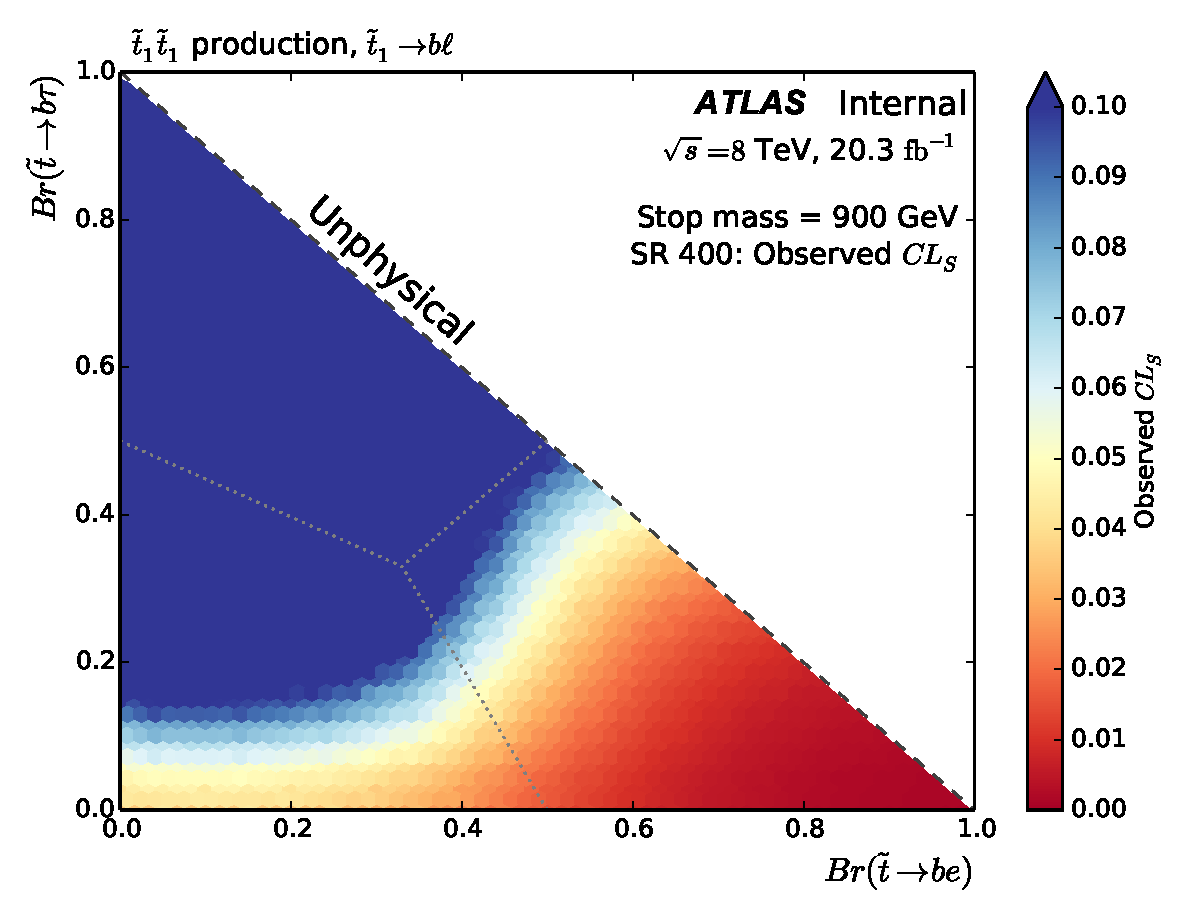
\includegraphics[width=0.65\textwidth]
      {figs/blstop/cls_plots/cls_vs_br_m_900_sr_400_obs.pdf}
  }
  \subbottom[Observed $CL_S$ for SR~600]{
    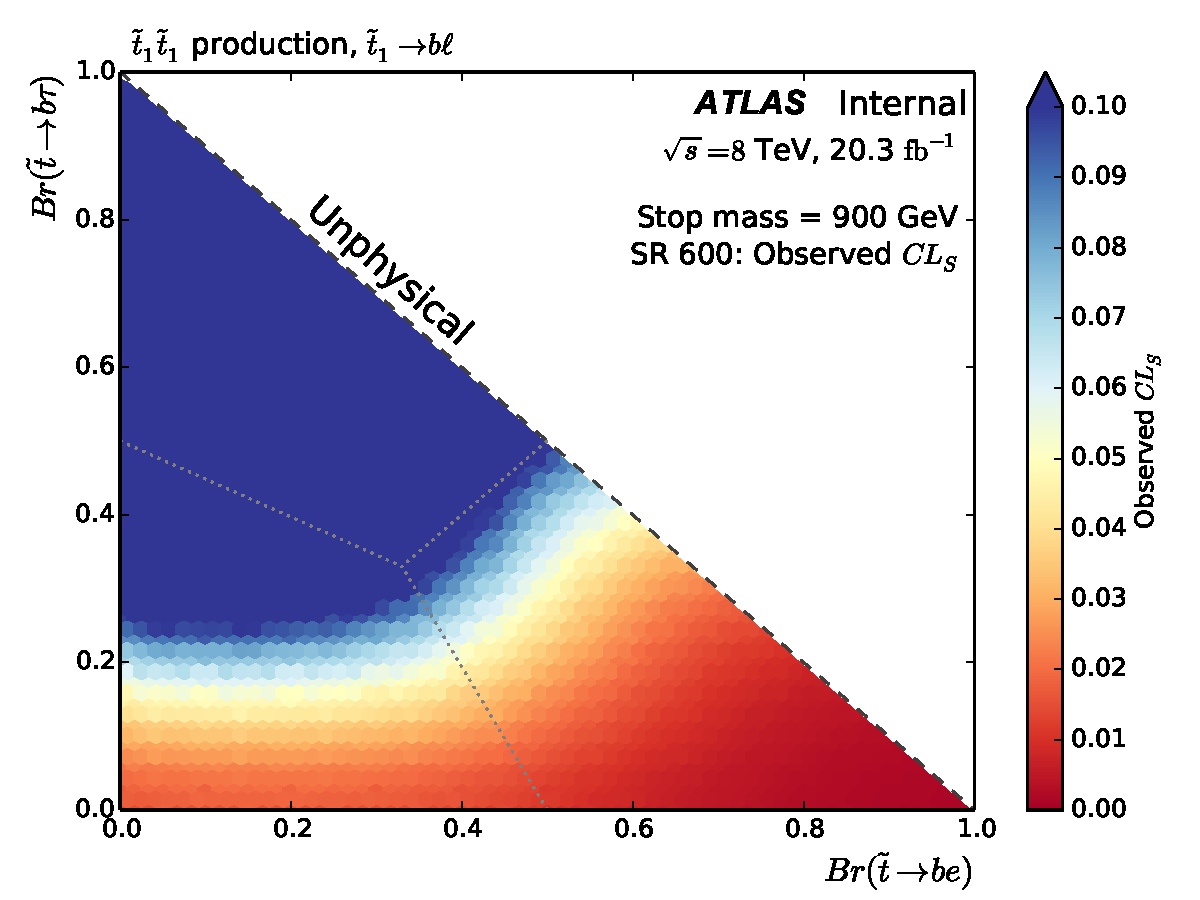
\includegraphics[width=0.65\textwidth]
      {figs/blstop/cls_plots/cls_vs_br_m_900_sr_600_obs.pdf}
  }
  \caption{
    Observed
    $CL_S$ values for SR~400 (top) and SR~600 (bottom) for a stop mass of
    900~\GeV,
    shown across the plane of physical stop branching ratios.
  }
\end{figure}

\begin{figure}[ht]
  \centering
  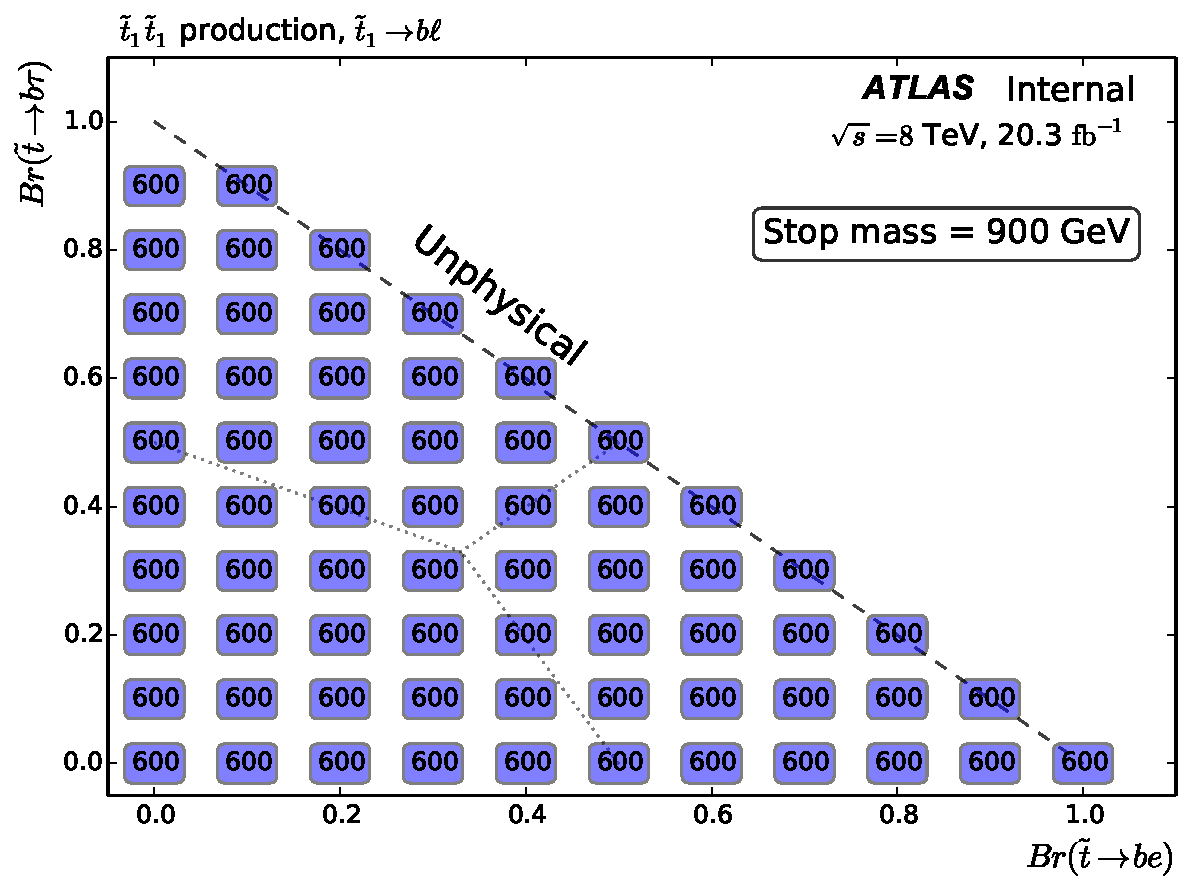
\includegraphics[width=0.85\textwidth]
    {figs/blstop/region_selection/region_choice_vs_br_m_900.pdf}
  \caption{
    SR selection for a stop mass of 900~\GeV.
  }
\end{figure}

\FloatBarrier

%% -----------------------------------------------------------------------------
\newpage
\section{1000 GeV stop mass}

\begin{figure}[ht]
  \centering
  \subbottom[Expected $CL_S$ for SR~400]{
    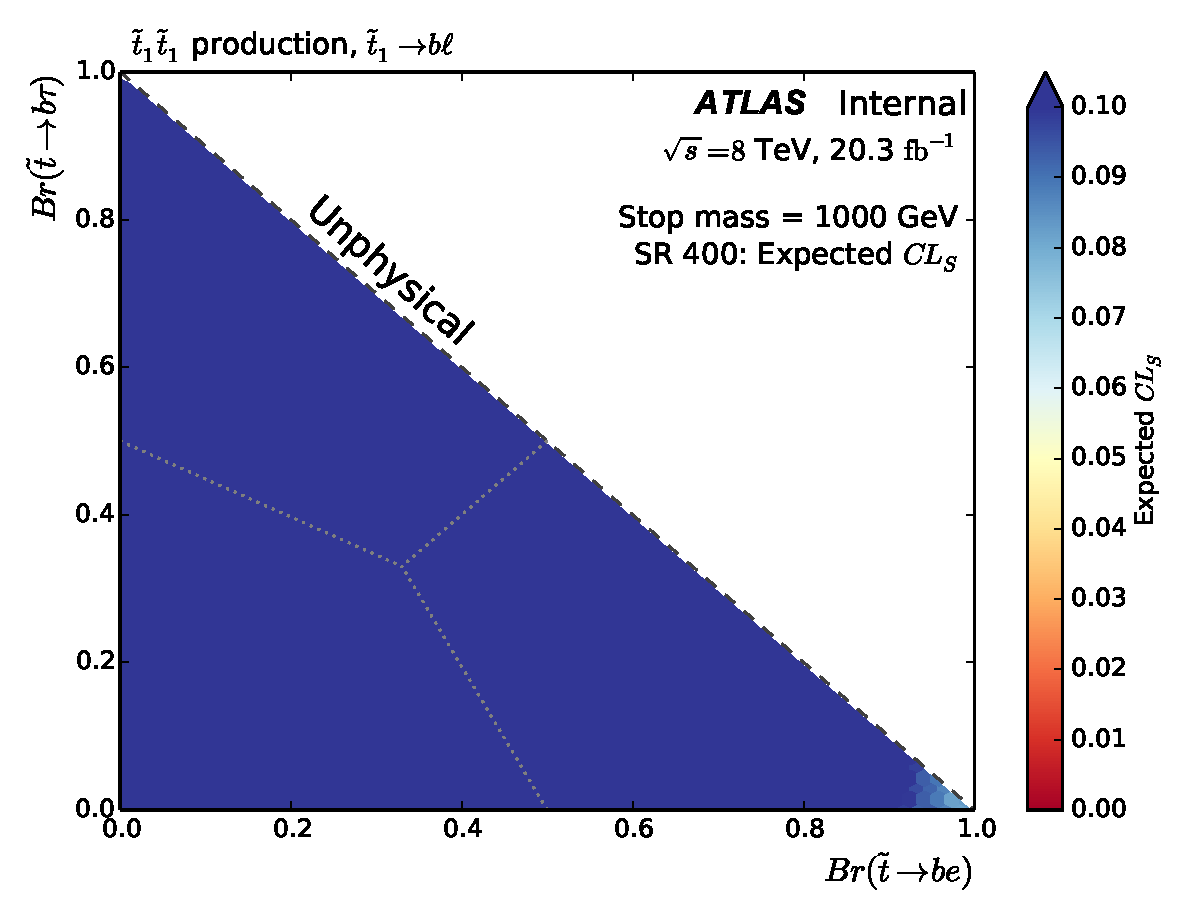
\includegraphics[width=0.65\textwidth]
      {figs/blstop/cls_plots/cls_vs_br_m_1000_sr_400_exp.pdf}
  }
  \subbottom[Expected $CL_S$ for SR~600]{
    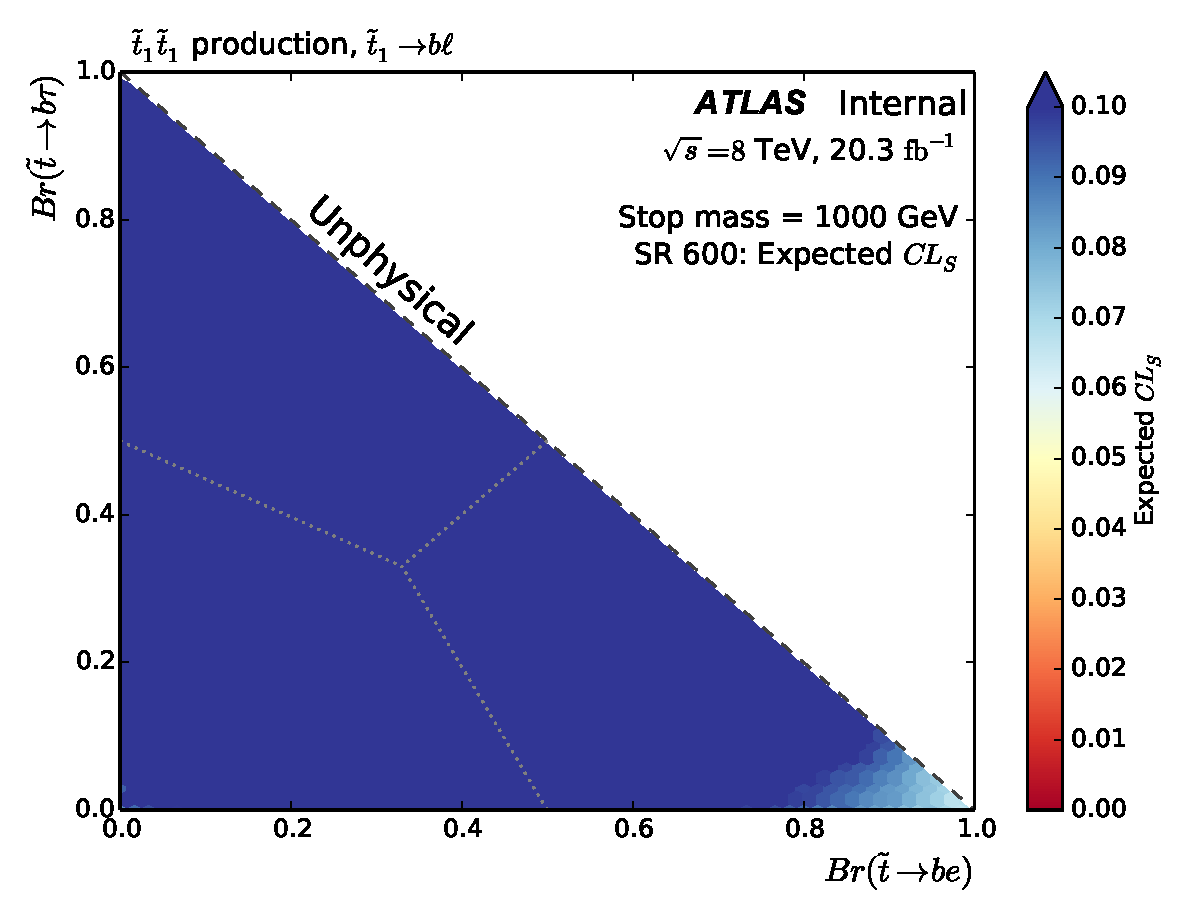
\includegraphics[width=0.65\textwidth]
      {figs/blstop/cls_plots/cls_vs_br_m_1000_sr_600_exp.pdf}
  }
  \caption{
    Expected
    $CL_S$ values for SR~400 (top) and SR~600 (bottom) for a stop mass of
    1~\TeV,
    shown across the plane of physical stop branching ratios.
  }
\end{figure}

\begin{figure}[ht]
  \centering
  \subbottom[Observed $CL_S$ for SR~400]{
    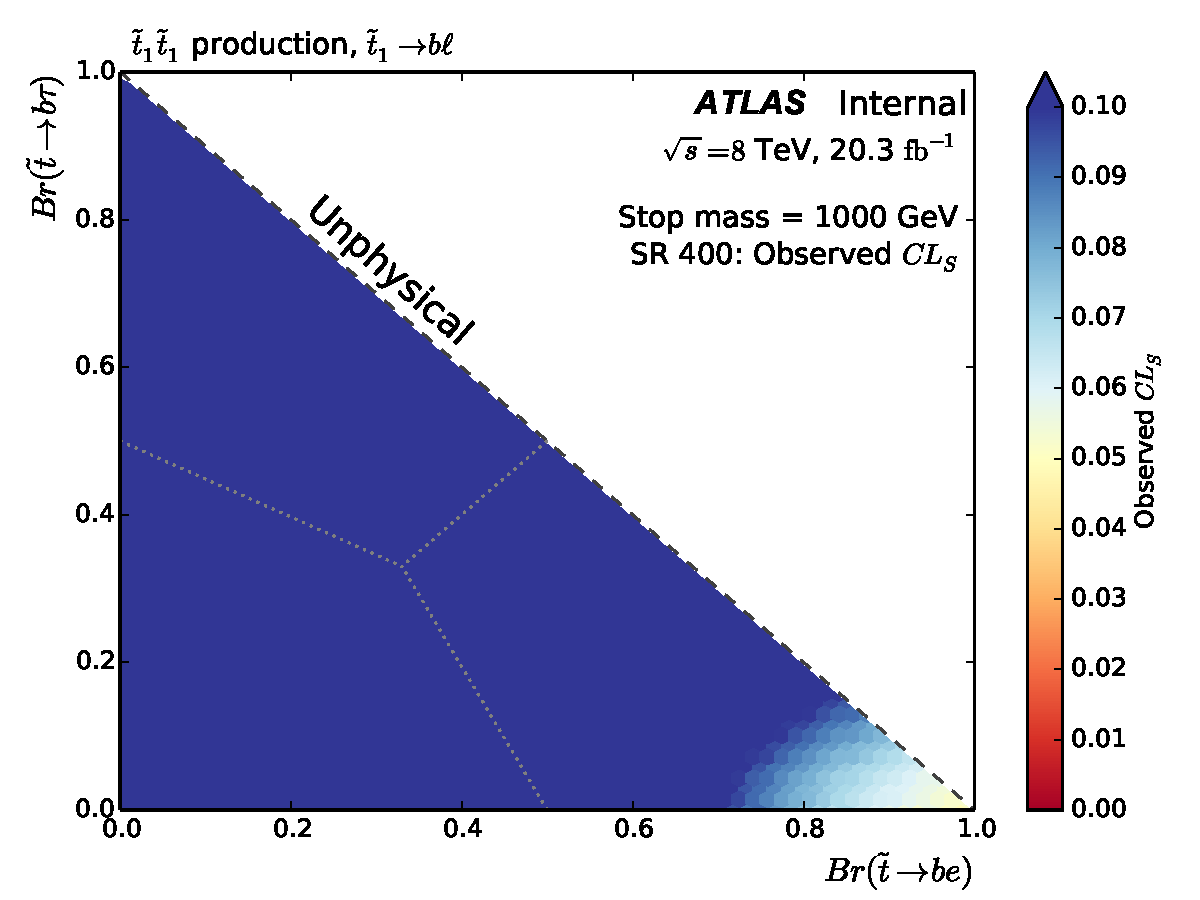
\includegraphics[width=0.65\textwidth]
      {figs/blstop/cls_plots/cls_vs_br_m_1000_sr_400_obs.pdf}
  }
  \subbottom[Observed $CL_S$ for SR~600]{
    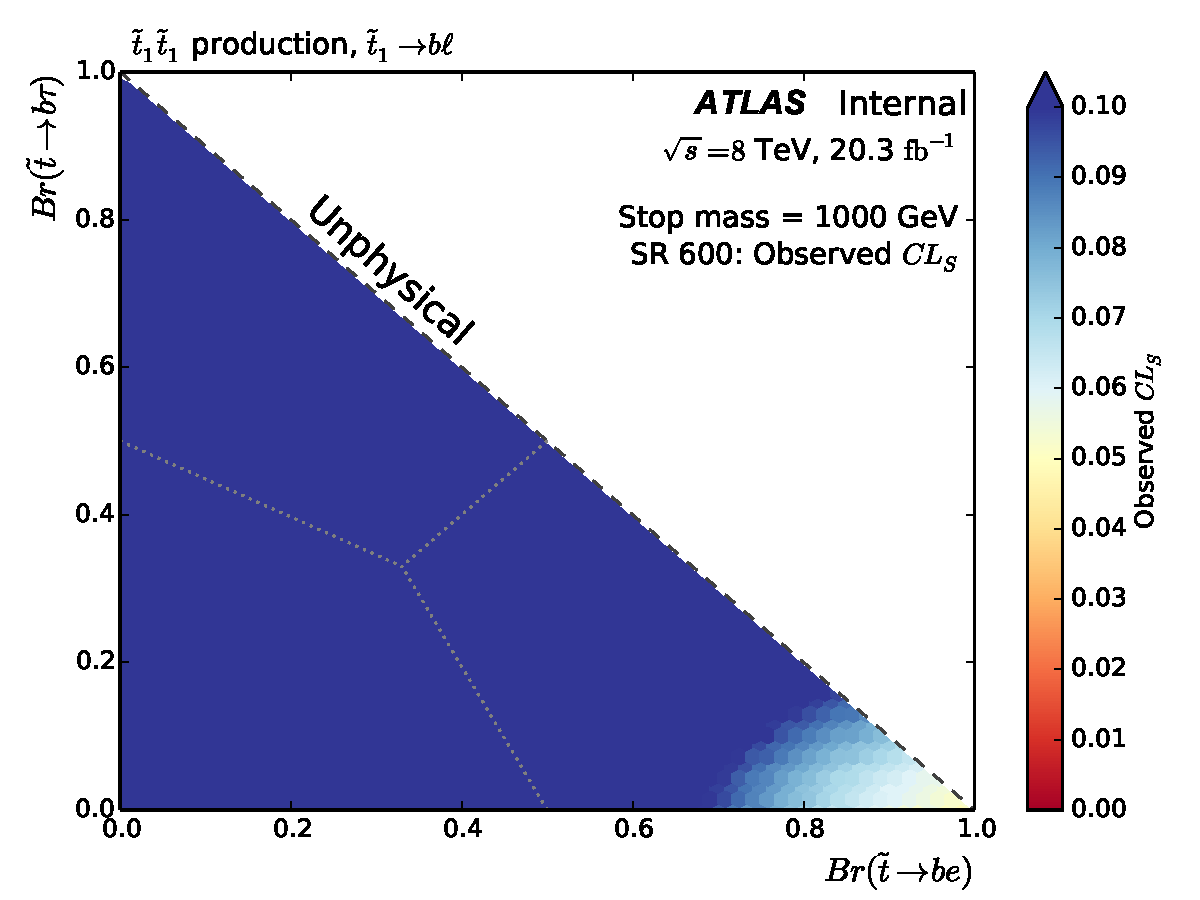
\includegraphics[width=0.65\textwidth]
      {figs/blstop/cls_plots/cls_vs_br_m_1000_sr_600_obs.pdf}
  }
  \caption{
    Observed
    $CL_S$ values for SR~400 (top) and SR~600 (bottom) for a stop mass of
    1~\TeV,
    shown across the plane of physical stop branching ratios.
  }
\end{figure}

\begin{figure}[ht]
  \centering
  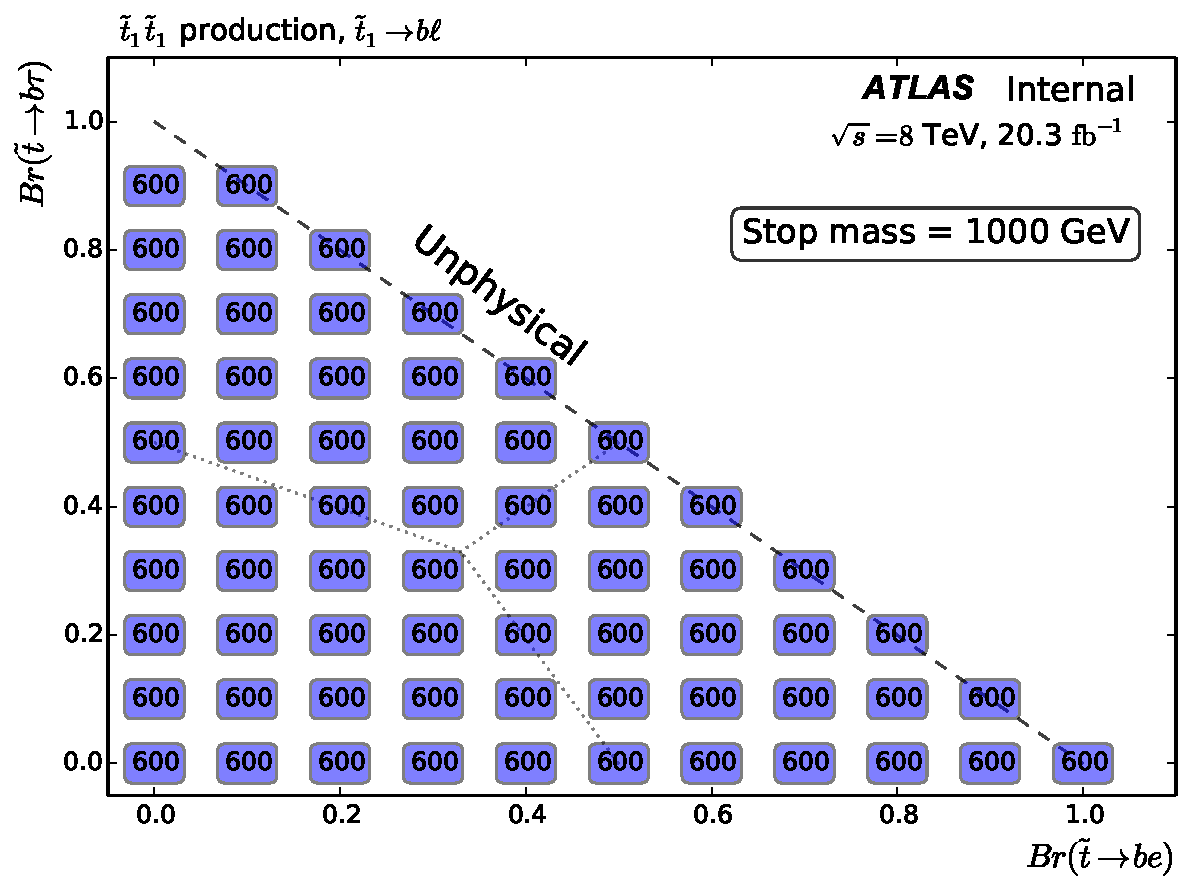
\includegraphics[width=0.85\textwidth]
    {figs/blstop/region_selection/region_choice_vs_br_m_1000.pdf}
  \caption{
    SR selection for a stop mass of 1~\TeV.
  }
\end{figure}

\FloatBarrier

%% -----------------------------------------------------------------------------
\newpage
\section{1100 GeV stop mass}

\begin{figure}[ht]
  \centering
  \subbottom[Expected $CL_S$ for SR~400]{
    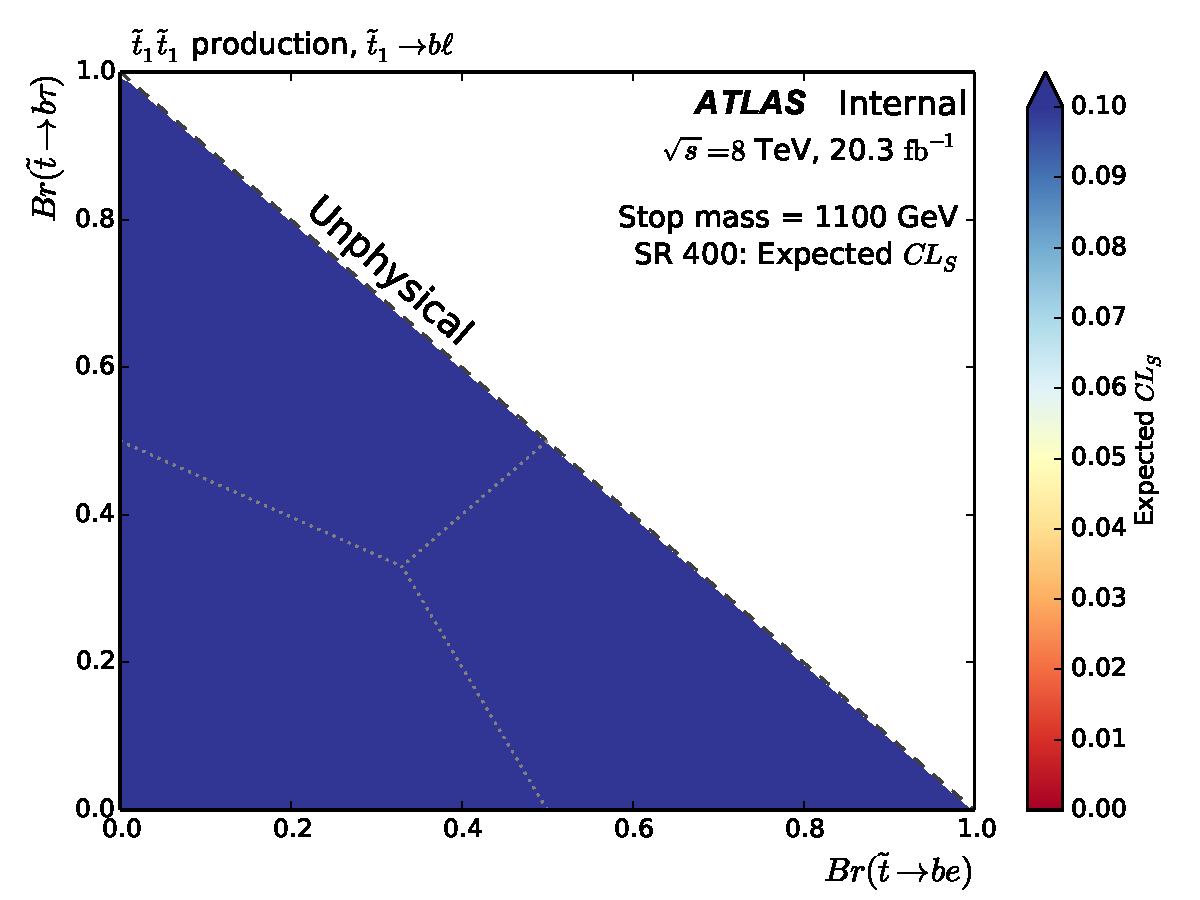
\includegraphics[width=0.65\textwidth]
      {figs/blstop/cls_plots/cls_vs_br_m_1100_sr_400_exp.pdf}
  }
  \subbottom[Expected $CL_S$ for SR~600]{
    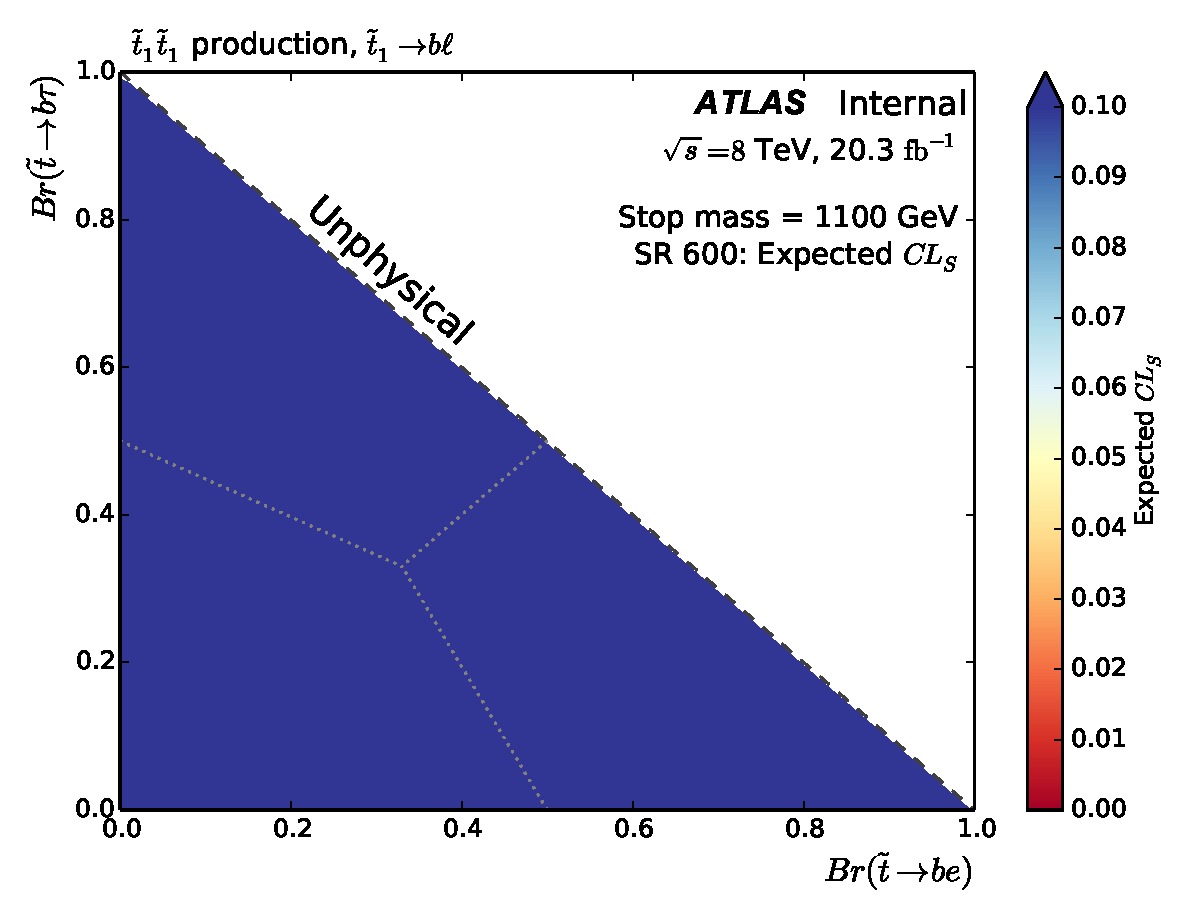
\includegraphics[width=0.65\textwidth]
      {figs/blstop/cls_plots/cls_vs_br_m_1100_sr_600_exp.pdf}
  }
  \caption{
    Expected
    $CL_S$ values for SR~400 (top) and SR~600 (bottom) for a stop mass of
    1.1~\TeV,
    shown across the plane of physical stop branching ratios.
  }
\end{figure}

\begin{figure}[ht]
  \centering
  \subbottom[Observed $CL_S$ for SR~400]{
    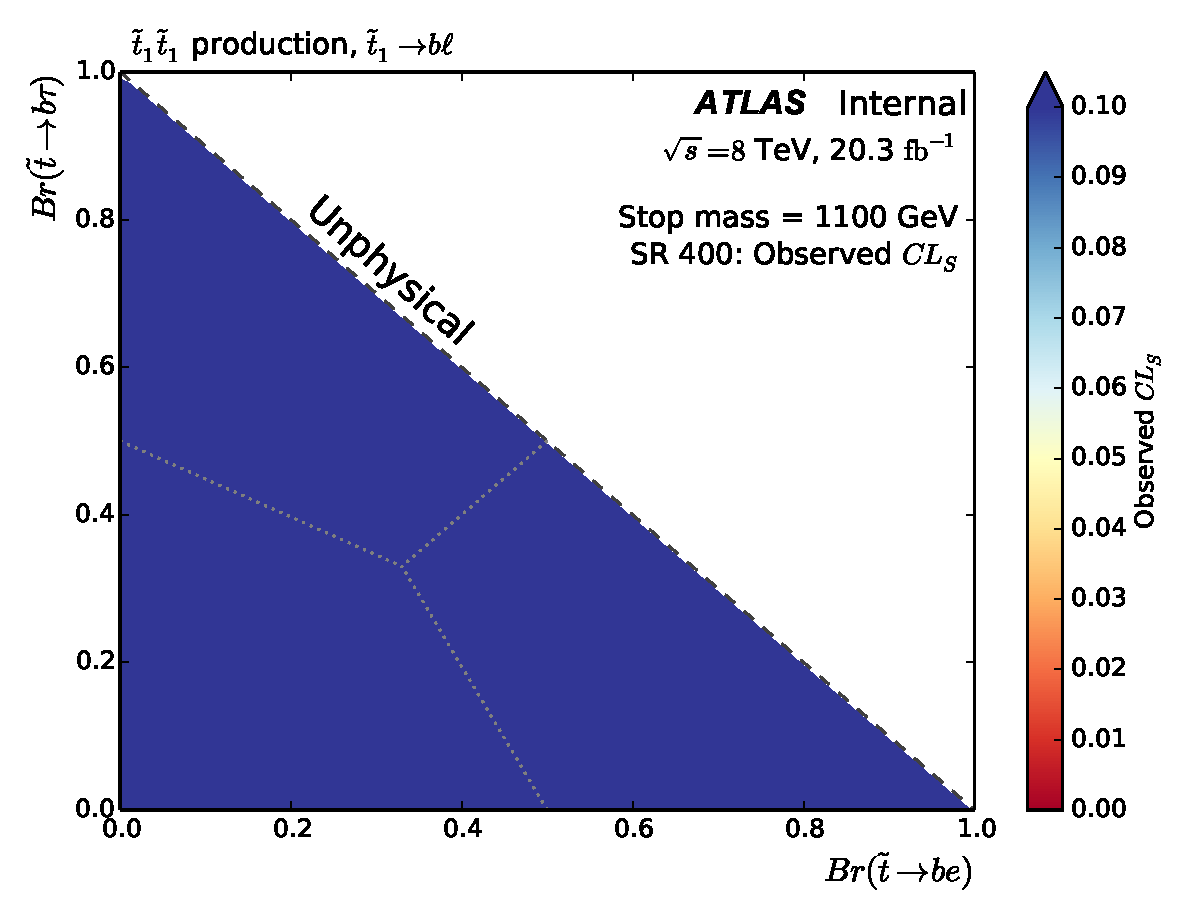
\includegraphics[width=0.65\textwidth]
      {figs/blstop/cls_plots/cls_vs_br_m_1100_sr_400_obs.pdf}
  }
  \subbottom[Observed $CL_S$ for SR~600]{
    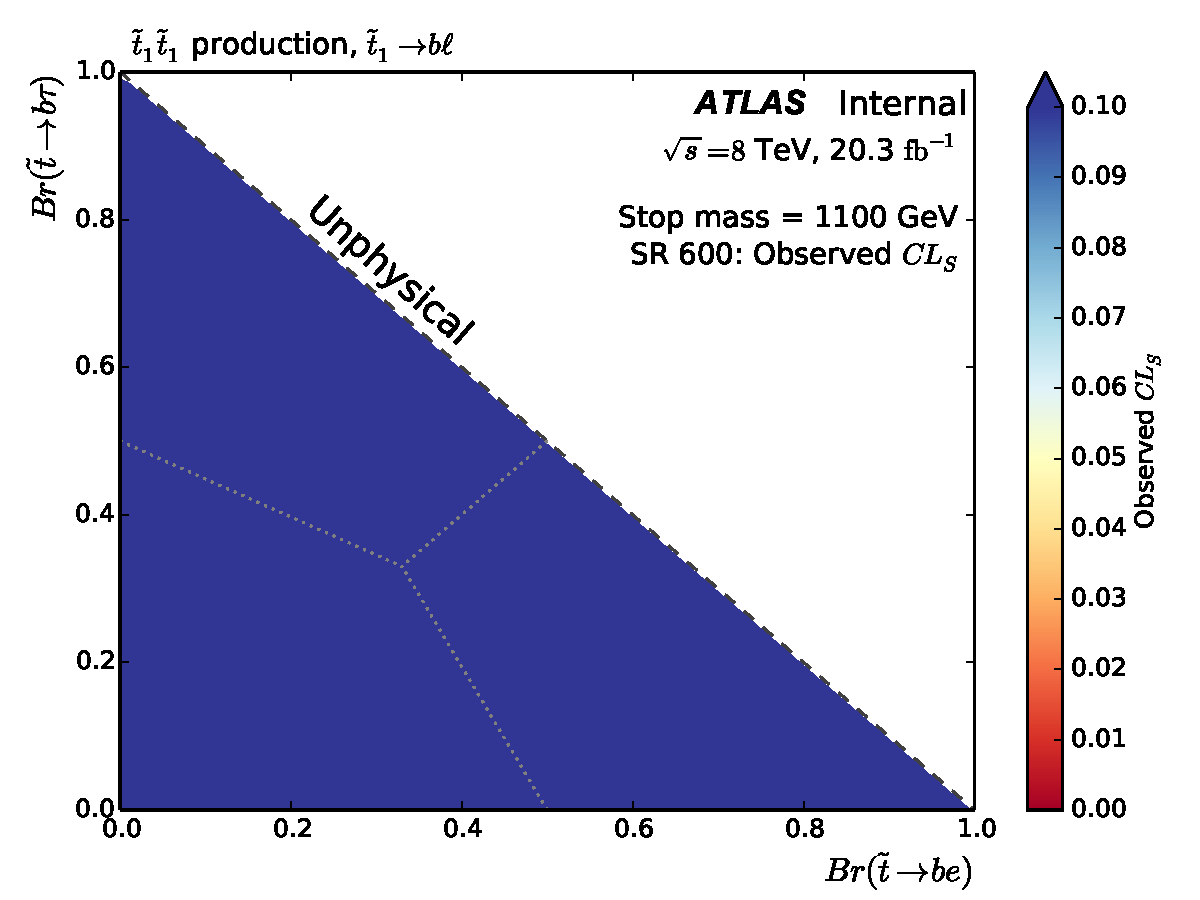
\includegraphics[width=0.65\textwidth]
      {figs/blstop/cls_plots/cls_vs_br_m_1100_sr_600_obs.pdf}
  }
  \caption{
    Observed
    $CL_S$ values for SR~400 (top) and SR~600 (bottom) for a stop mass of
    1.1~\TeV,
    shown across the plane of physical stop branching ratios.
  }
\end{figure}

\begin{figure}[ht]
  \centering
  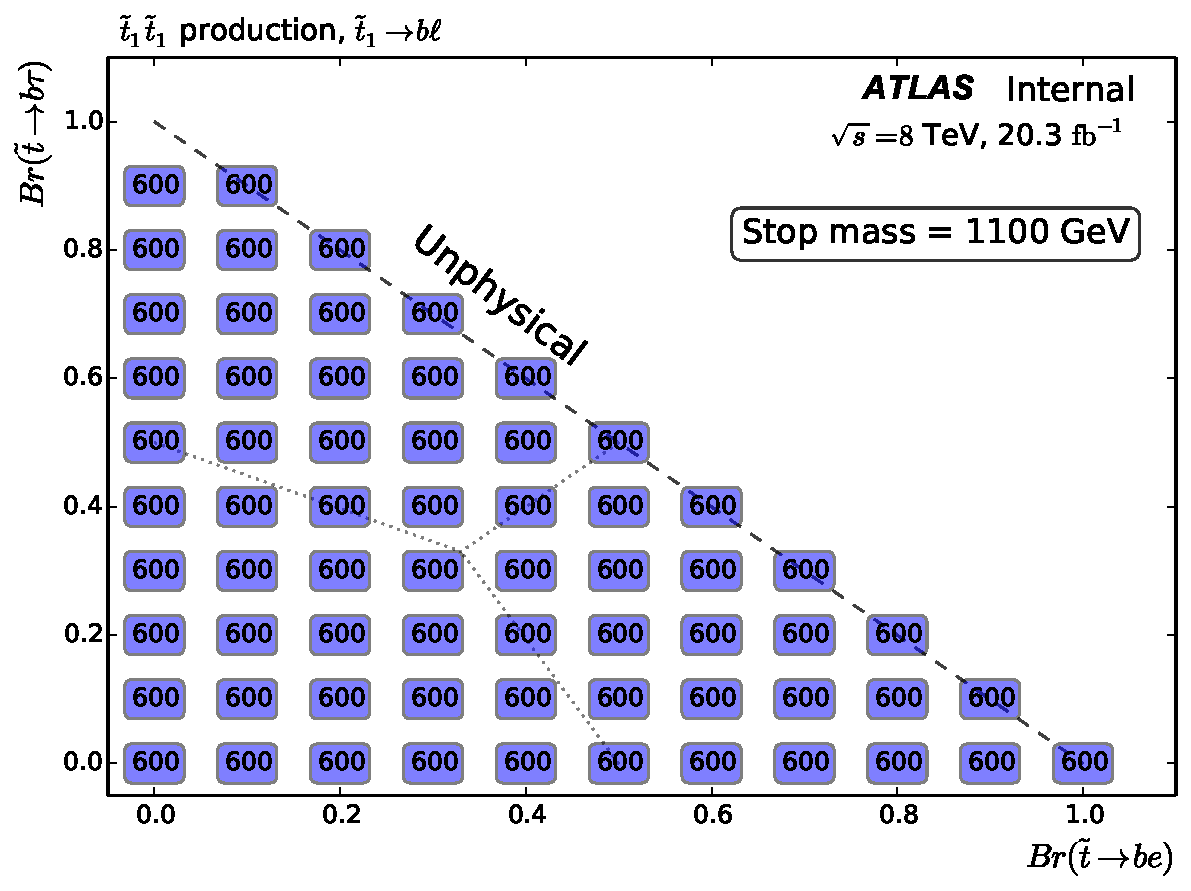
\includegraphics[width=0.85\textwidth]
    {figs/blstop/region_selection/region_choice_vs_br_m_1100.pdf}
  \caption{
    SR selection for a stop mass of 1.1~\TeV.
  }
\end{figure}

\FloatBarrier

%% \begin{figure}[ht]
%%   \centering
%%   \subbottom[Expected $CL_S$ for SR 400]{
%%     \includegraphics[width=0.48\textwidth]
%%       {figs/blstop/cls_plots/cls_vs_br_m_400_sr_400_exp.pdf}}
%%   \subbottom[Expected $CL_S$ for SR 600]{
%%     \includegraphics[width=0.48\textwidth]
%%       {figs/blstop/cls_plots/cls_vs_br_m_400_sr_600_exp.pdf}}
%%   % \subbottom[Selected region]{
%%   %   \includegraphics[width=0.48\textwidth]
%%   %     {figs/blstop/region_selection/region_choice_vs_br_m_400.pdf}}
%%   \caption{blah blah blah expected blah blah blah}
%% \end{figure}

% \begin{figure}[ht]
%   \centering
%   \subbottom[Observed $CL_S$ for SR 400]{
%     \includegraphics[width=0.40\textwidth]
%       {figs/blstop/cls_plots/cls_vs_br_m_400_sr_400_obs.pdf}}
%   \subbottom[Observed $CL_S$ for SR 600]{
%     \includegraphics[width=0.40\textwidth]
%       {figs/blstop/cls_plots/cls_vs_br_m_400_sr_600_obs.pdf}}
%   \caption{blah blah blah observed blah blah blah}
% \end{figure}

% \FloatBarrier


%% figs/blstop/cls_plots/cls_vs_br_m_500_sr_400_exp.pdf
%% figs/blstop/cls_plots/cls_vs_br_m_500_sr_400_obs.pdf
%% figs/blstop/cls_plots/cls_vs_br_m_500_sr_600_exp.pdf
%% figs/blstop/cls_plots/cls_vs_br_m_500_sr_600_obs.pdf
%% figs/blstop/cls_plots/cls_vs_br_m_600_sr_400_exp.pdf
%% figs/blstop/cls_plots/cls_vs_br_m_600_sr_400_obs.pdf
%% figs/blstop/cls_plots/cls_vs_br_m_600_sr_600_exp.pdf
%% figs/blstop/cls_plots/cls_vs_br_m_600_sr_600_obs.pdf
%% figs/blstop/cls_plots/cls_vs_br_m_700_sr_400_exp.pdf
%% figs/blstop/cls_plots/cls_vs_br_m_700_sr_400_obs.pdf
%% figs/blstop/cls_plots/cls_vs_br_m_700_sr_600_exp.pdf
%% figs/blstop/cls_plots/cls_vs_br_m_700_sr_600_obs.pdf
%% figs/blstop/cls_plots/cls_vs_br_m_800_sr_400_exp.pdf
%% figs/blstop/cls_plots/cls_vs_br_m_800_sr_400_obs.pdf
%% figs/blstop/cls_plots/cls_vs_br_m_800_sr_600_exp.pdf
%% figs/blstop/cls_plots/cls_vs_br_m_800_sr_600_obs.pdf
%% figs/blstop/cls_plots/cls_vs_br_m_900_sr_400_exp.pdf
%% figs/blstop/cls_plots/cls_vs_br_m_900_sr_400_obs.pdf
%% figs/blstop/cls_plots/cls_vs_br_m_900_sr_600_exp.pdf
%% figs/blstop/cls_plots/cls_vs_br_m_900_sr_600_obs.pdf
%% 
%% figs/blstop/cls_plots/cls_vs_br_m_1000_sr_400_exp.pdf
%% figs/blstop/cls_plots/cls_vs_br_m_1000_sr_400_obs.pdf
%% figs/blstop/cls_plots/cls_vs_br_m_1000_sr_600_exp.pdf
%% figs/blstop/cls_plots/cls_vs_br_m_1000_sr_600_obs.pdf
%% figs/blstop/cls_plots/cls_vs_br_m_1100_sr_400_exp.pdf
%% figs/blstop/cls_plots/cls_vs_br_m_1100_sr_400_obs.pdf
%% figs/blstop/cls_plots/cls_vs_br_m_1100_sr_600_exp.pdf
%% figs/blstop/cls_plots/cls_vs_br_m_1100_sr_600_obs.pdf
%% 
%% figs/blstop/region_selection/region_choice_vs_br_m_500.pdf
%% figs/blstop/region_selection/region_choice_vs_br_m_600.pdf
%% figs/blstop/region_selection/region_choice_vs_br_m_700.pdf
%% figs/blstop/region_selection/region_choice_vs_br_m_800.pdf
%% figs/blstop/region_selection/region_choice_vs_br_m_900.pdf
%% figs/blstop/region_selection/region_choice_vs_br_m_1000.pdf
%% figs/blstop/region_selection/region_choice_vs_br_m_1100.pdf
